% Relatório do projeto -- CIN0114 (2026.2), Equipe 10
% Reprodução do GraphIDS (Guerra et al., NeurIPS 2025) e avaliação no NF-ToN-IoT-v3.
%
% Compilação (na pasta relatorio/):
%   latexmk -pdf main.tex
% As tabelas em tabelas/ são geradas por gerar_tabelas.py a partir de results/.
\documentclass[conference,a4paper]{IEEEtran}

\usepackage[utf8]{inputenc}
\usepackage[T1]{fontenc}
\usepackage[brazil]{babel}
\usepackage{amsmath,amssymb}
\usepackage{graphicx}
\usepackage{booktabs}
\usepackage{multirow}
\usepackage{makecell}
\usepackage{array}
\usepackage{xcolor}
\usepackage[portuguese,ruled,vlined,linesnumbered]{algorithm2e}
\usepackage{tikz}
\usetikzlibrary{arrows.meta,positioning,fit,shapes.geometric,calc,backgrounds}
\usepackage{cite}
\usepackage{url}
\usepackage[hidelinks]{hyperref}

\graphicspath{{figuras/}}

\newcommand{\vect}[1]{\mathbf{#1}}
\newcommand{\norm}[1]{\left\lVert #1 \right\rVert}
\renewcommand{\arraystretch}{1.1}

\begin{document}

\title{Reprodução e Avaliação do GraphIDS:\\ Detecção Auto-Supervisionada de Intrusão em Rede\\ com Representações de Grafos}

\author{
\IEEEauthorblockN{Rafael Xavier, Danilo Barrote, Bernardo Siqueira Batista e Felipe Maran Alves}
\IEEEauthorblockA{Centro de Informática (CIn), Universidade Federal de Pernambuco (UFPE)\\
CIN0114 -- Técnicas de Ataque e Detecção de Intrusão, 2026.2 -- Equipe 10\\
Recife, Brasil}
}

\maketitle

% ----------------------------------------------------------------------------
\begin{abstract}
Sistemas de detecção de intrusão em rede (NIDS) baseados em aprendizado
supervisionado dependem de grandes volumes de tráfego rotulado e tendem a falhar
diante de ataques que não aparecem no treino. Métodos auto-supervisionados com
redes neurais de grafos (GNNs), como o Anomal-E, evitam os rótulos de ataque, mas
separam o aprendizado das representações da etapa de detecção. O GraphIDS (Guerra
\emph{et al.}, NeurIPS 2025) une as duas etapas: o tráfego NetFlow é modelado como
um grafo de hosts e fluxos, um E-GraphSAGE gera um embedding por fluxo com o
contexto local de 1 salto e um autoencoder Transformer com máscara de atenção
aprende a reconstruir esses embeddings a partir apenas de tráfego benigno; o erro
de reconstrução é o score de anomalia. Neste trabalho, reimplementamos o GraphIDS
do zero em PyTorch, sem bibliotecas de grafos, e o avaliamos nos quatro datasets
do artigo (NF-UNSW-NB15 e NF-CSE-CIC-IDS2018, versões 2 e 3) e num dataset novo,
o NF-ToN-IoT-v3, de um ambiente IoT/IIoT. Com três seeds por dataset, a
reprodução fica a até dois desvios-padrão do valor publicado em 7 das 8 métricas,
com PR-AUC de 0,9983 e F1 macro de 0,9999 no NF-UNSW-NB15-v3. No NF-ToN-IoT-v3 o
desempenho cai para PR-AUC de 0,6872 e F1 macro de 0,6408: ataques como backdoor
e ransomware são sempre detectados, mas varreduras e boa parte dos ataques web e
de negação de serviço são reconstruídos tão bem quanto o tráfego benigno, o que
expõe limites do método quando os ataques compartilham os hosts do tráfego
normal e são muito frequentes.
\end{abstract}

\begin{IEEEkeywords}
detecção de intrusão, redes neurais de grafos, aprendizado auto-supervisionado,
autoencoder mascarado, Transformer, NetFlow, reprodutibilidade
\end{IEEEkeywords}

% ----------------------------------------------------------------------------
\section{Introdução}
\label{sec:introducao}

\textbf{Problema.} Este trabalho investiga a detecção de intrusões em tráfego de
rede a partir de registros de fluxo (NetFlow): dado um conjunto de fluxos
observados entre hosts, decidir quais deles pertencem a um ataque. A dificuldade
está em fazer isso com pouca ou nenhuma supervisão, porque ataques novos surgem o
tempo todo e rotular tráfego é caro e exige especialistas.

\textbf{Por que é interessante.} O número de dispositivos conectados e a
sofisticação dos ataques crescem continuamente, de redes corporativas a ambientes
IoT. NIDS supervisionados aprendem as assinaturas estatísticas dos ataques vistos
no treino e generalizam mal para ataques desconhecidos, além de precisarem de
retreino frequente~\cite{sommer2010outside,maseer2021benchmarking}. Uma abordagem
que aprende apenas o comportamento normal da rede e sinaliza desvios
(\emph{detecção de anomalias}) não depende de rótulos de ataque e, em princípio,
pode detectar ataques nunca vistos.

\textbf{Soluções existentes e desvantagens.} Detectores de anomalia clássicos
(CBLOF, Isolation Forest, HBOS) e autoencoders aplicados às features de cada fluxo
isolado~\cite{he2003cblof,liu2008iforest,mirsky2018kitsune} ignoram a estrutura
de comunicação entre hosts, que é justamente o que caracteriza varreduras,
ataques distribuídos e botnets. GNNs como o E-GraphSAGE~\cite{lo2022egraphsage}
exploram essa estrutura, mas são treinadas de forma supervisionada. O
Anomal-E~\cite{caville2022anomale} remove a necessidade de rótulos com um pré-treino
contrastivo, porém (i) separa o aprendizado das representações da detecção, de
modo que os embeddings não são otimizados para a tarefa final, e (ii) depende de
amostras negativas construídas artificialmente. O SAFE~\cite{li2025safe} usa um
autoencoder mascarado sobre features tabulares transformadas em imagens, sem
nenhuma informação topológica.

\textbf{Por que o artigo de referência propôs o GraphIDS.} Guerra
\emph{et al.}~\cite{guerra2025graphids} argumentam que, em detecção de intrusão,
a informação relevante está nas arestas (fluxos) e no seu contexto local, e que os
embeddings devem ser aprendidos \emph{para} a detecção. O GraphIDS treina de ponta
a ponta um E-GraphSAGE e um autoencoder Transformer com máscara de atenção para
reconstruir representações de tráfego benigno; o erro de reconstrução de cada
fluxo é o seu score de anomalia. O treino usa apenas fluxos benignos e dispensa
amostras negativas.

\textbf{O que este trabalho propõe.} Reproduzimos o GraphIDS com uma implementação
própria, feita do zero, e avaliamos sua capacidade de generalização num ambiente
diferente dos usados pelos autores. As principais contribuições são:
\begin{itemize}
  \item uma reimplementação completa e comentada do GraphIDS em PyTorch puro,
        incluindo a amostragem de vizinhança, sem DGL nem PyTorch Geometric,
        disponível publicamente com testes automatizados~\cite{equipe10_repo};
  \item a reprodução dos resultados nos quatro datasets do artigo com três
        seeds cada, em que 7 das 8 métricas ficam a até dois desvios-padrão
        dos valores publicados;
  \item a primeira avaliação do GraphIDS no NF-ToN-IoT-v3, um dataset IoT/IIoT
        com alta prevalência de ataques e categorias que o artigo não cobre;
  \item uma análise por categoria de ataque, por seed, de custo computacional e
        das representações aprendidas (t-SNE), que explica onde o método
        funciona e onde falha.
\end{itemize}

O restante do texto está organizado assim: a Seção~\ref{sec:relacionados}
discute trabalhos relacionados; a Seção~\ref{sec:ameaca}, o modelo de ameaça; a
Seção~\ref{sec:sistema}, o sistema do artigo de referência; a
Seção~\ref{sec:proposta}, a proposta de melhoria; a
Seção~\ref{sec:metodologia}, os dados, as métricas e os experimentos; a
Seção~\ref{sec:resultados}, os resultados; e a Seção~\ref{sec:conclusao}, as
conclusões.

% ----------------------------------------------------------------------------
\section{Trabalhos relacionados}
\label{sec:relacionados}

\textbf{Modelagem mascarada auto-supervisionada.} O BERT~\cite{devlin2019bert}
aprende representações de texto reconstruindo tokens mascarados, e os masked
autoencoders (MAE)~\cite{he2022mae} fazem o mesmo com blocos de imagem. O
GraphMAE~\cite{hou2022graphmae} leva a ideia para grafos, reconstruindo features
de nós mascarados. Como anomalias tendem a ser mal reconstruídas, esse paradigma
foi adaptado à detecção de anomalias, por exemplo em logs de sistema com o
LogBERT~\cite{guo2021logbert}. A limitação comum é que nenhum desses modelos foi
pensado para dados em que a informação principal está nas arestas, como fluxos
de rede.

\textbf{GNNs para detecção supervisionada.} GCN~\cite{kipf2017gcn} e
GraphSAGE~\cite{hamilton2017graphsage} aprendem embeddings de nós agregando a
vizinhança; o GraphSAGE é indutivo, ou seja, gera embeddings para nós não vistos
no treino. O E-GraphSAGE~\cite{lo2022egraphsage} incorpora features de arestas na
troca de mensagens e classifica fluxos NetFlow com alto desempenho em datasets
IoT. Friji \emph{et al.}~\cite{friji2023flowgraph} propõem um grafo em que cada
fluxo é um nó, o que torna visíveis padrões de ataques em várias etapas, e Zhou
\emph{et al.}~\cite{zhou2020botnet} detectam botnets usando apenas a topologia.
Todos dependem de tráfego rotulado, o que limita o uso em ambientes reais.

\textbf{GNNs para detecção auto-supervisionada.} O
Anomal-E~\cite{caville2022anomale} pré-treina um E-GraphSAGE com uma variante do
Deep Graph Infomax~\cite{velickovic2019dgi} e aplica detectores clássicos (PCA,
Isolation Forest, CBLOF, HBOS) sobre os embeddings. As duas etapas são
independentes, e o pré-texto contrastivo exige amostras negativas geradas por
embaralhamento. Além disso, a implementação pública usa \emph{target encoding}
com rótulos de ataque e escolhe o detector pelo teste, o que os autores do
GraphIDS corrigiram na comparação~\cite{guerra2025graphids}.

\textbf{Autoencoders para NIDS.} O Kitsune~\cite{mirsky2018kitsune} usa um
conjunto de autoencoders sobre estatísticas incrementais de pacotes e o
SAFE~\cite{li2025safe} combina um MAE convolucional com um detector LOF. Ambos
tratam cada amostra isoladamente, sem o contexto de comunicação entre hosts, e o
SAFE perde muito desempenho nos datasets maiores (Tabela~\ref{tab:reproducao}).

% ----------------------------------------------------------------------------
\section{Modelo de ameaça}
\label{sec:ameaca}

\textbf{Cenário.} O defensor protege uma rede (corporativa, no UNSW-NB15 e no
CSE-CIC-IDS2018, ou IoT/IIoT, no ToN-IoT) e tem um ponto de observação, como um
roteador ou \emph{switch} de borda, que exporta registros NetFlow para um coletor
(Figura~\ref{fig:ameaca}). O GraphIDS roda sobre os fluxos coletados e marca como
suspeitos os que fogem do padrão aprendido. O atacante pode ser externo, enviando
tráfego da Internet para a rede, ou interno, controlando um host já comprometido
(por e-mail malicioso, \emph{backdoor} ou \emph{bot}).

\begin{figure}[t]
\centering
\begin{tikzpicture}[
  font=\scriptsize,
  host/.style={draw, rounded corners=2pt, minimum width=0.9cm, minimum height=0.45cm, fill=blue!6},
  bad/.style={draw, rounded corners=2pt, minimum width=0.9cm, minimum height=0.45cm, fill=red!12},
  box/.style={draw, rounded corners=2pt, align=center, fill=gray!8},
  >=Stealth]
  \node[bad] (ext) at (0,1.6) {Atacante};
  \node[box, minimum width=1.2cm] (inet) at (0,0.5) {Internet};
  \node[box, minimum width=1.7cm] (rt) at (2.1,0.5) {Roteador /\\exportador NetFlow};
  \node[host] (h1) at (4.3,1.5) {Host A};
  \node[host] (h2) at (4.3,0.85) {Host B};
  \node[host] (h3) at (4.3,0.2) {Servidor};
  \node[bad]  (h4) at (4.3,-0.45) {Host comp.};
  \node[box, minimum width=1.6cm] (col) at (2.1,-1.0) {Coletor de\\fluxos};
  \node[box, minimum width=1.6cm, fill=green!10] (ids) at (0,-1.0) {GraphIDS\\(score + limiar)};
  \draw[->, red!70!black, thick] (ext) -- (inet);
  \draw[<->] (inet) -- (rt);
  \foreach \h in {h1,h2,h3,h4} \draw[<->] (rt.east) -- (\h.west);
  \draw[->, red!70!black, thick, dashed] (h4.east) to[bend right=50] node[right, font=\tiny, align=left]{mov.\\lateral} (h1.east);
  \draw[->, dashed] (rt) -- node[right]{fluxos} (col);
  \draw[->] (col) -- (ids);
  \begin{scope}[on background layer]
    \node[draw, dotted, inner sep=4pt, fit=(rt)(h1)(h4)(col), label={[font=\tiny]below:rede monitorada}] {};
  \end{scope}
\end{tikzpicture}
\caption{Modelo de ameaça: o atacante age de fora ou a partir de um host comprometido; todo tráfego que passa pelo ponto de observação vira registro NetFlow, que é analisado pelo GraphIDS.}
\label{fig:ameaca}
\end{figure}

\textbf{Representação do tráfego.} Seja $G=(V,E)$ o grafo dirigido em que cada nó
$v\in V$ é um endereço IP e cada aresta $e=(u,v)\in E$ é um fluxo de $u$ para $v$
com vetor de features $\vect{x}_{uv}\in\mathbb{R}^F$ (bytes, pacotes, duração,
portas, protocolo, flags TCP etc.). Os graus de entrada e saída de um host são
\begin{equation}
d^{-}(v)=\left|\{(u,v)\in E\}\right|,\qquad d^{+}(u)=\left|\{(u,v)\in E\}\right|.
\end{equation}
Os ataques considerados deixam assinaturas diferentes nesse grafo:

\begin{itemize}
  \item \emph{Varredura e reconhecimento} (Reconnaissance, scanning): um atacante
        $a$ contata muitos destinos ou portas com fluxos curtos, de poucos
        pacotes: $d^{+}(a)\gg \mathbb{E}[d^{+}]$ e
        $\left|\{v:(a,v)\in E\}\right|$ grande.
  \item \emph{Negação de serviço} (DoS, DDoS, Hulk, Slowloris, LOIC, HOIC): um
        conjunto de origens $S$ envia fluxos a uma vítima $v$ a uma taxa
        $\lambda$ alta; $|S|=1$ no DoS e $|S|\gg 1$ no DDoS, de modo que
        $d^{-}(v)$ cresce rapidamente. Variantes lentas (Slowloris,
        SlowHTTPTest) mantêm conexões longas com pouquíssimos bytes.
  \item \emph{Força bruta} (SSH, FTP, password, ataques web de força bruta):
        muitos fluxos quase idênticos $\vect{x}_{av}\approx\vect{x}_{av}'$ entre
        o mesmo par $(a,v)$ e a mesma porta de serviço.
  \item \emph{Ataques à aplicação} (injection, SQL injection, XSS, Exploits,
        Shellcode, Fuzzers): o padrão de conexão é parecido com o de clientes
        legítimos (cliente $\to$ porta HTTP), e a diferença está no conteúdo, que
        o NetFlow só reflete indiretamente (tamanhos, duração, códigos).
  \item \emph{Comprometimento e movimento lateral} (Infiltration, Backdoor, Bot,
        ransomware, Worms, MITM): um host interno $c$ passa a ter arestas que
        não existiam no comportamento normal, como $c\to$ servidor de comando e
        controle ou varreduras internas. Quando o tráfego imita o benigno, a
        assinatura no grafo é fraca.
\end{itemize}

\textbf{Premissas.} Para que os ataques sejam executáveis e detectáveis no cenário
acima, assumimos que: (P1) o atacante consegue enviar tráfego à rede ou já
controla um host interno; (P2) o tráfego de ataque passa pelo ponto de
observação e gera registros NetFlow; (P3) os endereços IP identificam os hosts de
forma estável durante a janela observada (sem NAT ou \emph{spoofing}
sistemático que misture hosts); (P4) o tráfego usado no treino é benigno, isto
é, não há envenenamento dos dados de treino; (P5) o atacante não conhece o
modelo e não adapta o tráfego para imitar o comportamento normal (não
consideramos evasão adversarial); e (P6) existe um pequeno conjunto rotulado de
validação, usado apenas para escolher o checkpoint e o limiar.

% ----------------------------------------------------------------------------
\section{Sistema proposto pelo artigo de referência}
\label{sec:sistema}

O GraphIDS~\cite{guerra2025graphids} tem quatro componentes, ligados como na
Figura~\ref{fig:arquitetura}: (1) construção do grafo, (2) codificador
E-GraphSAGE, (3) autoencoder Transformer com máscara de atenção e (4) score de
anomalia com limiar.

\begin{figure*}[t]
\centering
\resizebox{\textwidth}{!}{%
\begin{tikzpicture}[
  font=\footnotesize,
  blk/.style={draw, rounded corners=3pt, align=center, minimum height=1.05cm, inner sep=3pt, fill=gray!7},
  gnn/.style={blk, fill=blue!8},
  tr/.style={blk, fill=orange!10},
  outb/.style={blk, fill=green!10},
  >=Stealth, node distance=0.55cm]
  \node[blk] (csv) {Fluxos NetFlow\\$\{(u,v,\vect{x}_{uv})\}$};
  \node[blk, right=of csv] (pre) {Limpeza, split\\80/10/10 e\\Min-Max};
  \node[blk, right=of pre] (graph) {Grafo dirigido\\hosts = nós\\fluxos = arestas};
  \node[gnn, right=of graph] (sage) {E-GraphSAGE\\(1 salto, \emph{fanout} $K$)\\$\vect{h}_{uv}\in\mathbb{R}^{d_{gnn}}$};
  \node[tr, right=of sage] (proj) {Projeção\\$\mathbb{R}^{d_{gnn}}\!\to\!\mathbb{R}^{d_{model}}$\\janelas de 512};
  \node[tr, right=of proj] (encdec) {Encoder + decoder\\Transformer\\(máscara $\vect{M}$ no treino)};
  \node[outb, right=of encdec] (score) {$s_i=\norm{\vect{h}_i-\hat{\vect{h}}_i}^2$\\ataque se $s_i>\tau$};
  \draw[->] (csv) -- (pre);
  \draw[->] (pre) -- (graph);
  \draw[->] (graph) -- (sage);
  \draw[->] (sage) -- (proj);
  \draw[->] (proj) -- (encdec);
  \draw[->] (encdec) -- (score);
  \draw[->, dashed, red!70!black] (score.south) -- ++(0,-0.45) -| node[pos=0.25, below, font=\scriptsize]{gradiente de $\mathcal{L}_{MSE}$ (treino só com fluxos benignos)} (sage.south);
\end{tikzpicture}}
\caption{Arquitetura do GraphIDS. O E-GraphSAGE e o Transformer são treinados juntos: o gradiente do erro de reconstrução atualiza os dois componentes.}
\label{fig:arquitetura}
\end{figure*}

\subsection{Construção do grafo}

\emph{Entrada:} tabela de fluxos NetFlow. \emph{Saída:} um grafo dirigido por
partição (treino, validação e teste). Cada IP vira um nó e cada fluxo uma aresta
dirigida da origem para o destino, cujas features são as colunas NetFlow menos os
IPs (e, nos datasets v3, menos os timestamps). As arestas de partições diferentes
não se misturam, mas o mapa IP~$\to$~nó é comum às três. Como os hosts não têm
atributos próprios, toda a informação está nas arestas.

\subsection{Codificador E-GraphSAGE}

\emph{Entrada:} um lote de arestas e a vizinhança amostrada. \emph{Saída:} um
embedding $\vect{h}_{uv}\in\mathbb{R}^{d_{gnn}}$ por fluxo (\texttt{edim\_out} na
Tabela~\ref{tab:hiper}). O E-GraphSAGE~\cite{lo2022egraphsage} é indutivo: aprende
funções de agregação em vez de depender de uma matriz de adjacência fixa, então
gera embeddings para hosts e fluxos que não estavam no grafo de treino. Com um
único salto e agregação por média, para cada host $w$ se calcula
\begin{align}
\vect{a}_w &= \frac{1}{|\mathcal{N}_K(w)|}\sum_{(z,w)\in\mathcal{N}_K(w)} \vect{x}_{zw}, \label{eq:agg}\\
\vect{h}_w &= \mathrm{ReLU}\left(\vect{W}_n\vect{a}_w+\vect{b}_n\right),\\
\vect{h}_{uv} &= \mathrm{Dropout}\left(\vect{W}_e\left[\vect{h}_u \,\Vert\, \vect{h}_v\right]+\vect{b}_e\right), \label{eq:edge}
\end{align}
em que $\mathcal{N}_K(w)$ são até $K$ arestas que chegam em $w$ (amostragem de
vizinhança com \emph{fanout} $K=32.768$) e $\Vert$ é a concatenação. A
restrição a um salto é deliberada: o contexto imediato já revela conexões
incomuns e rajadas, e o padrão global fica a cargo do Transformer, sem o custo de
GNNs mais profundas (o artigo valida a escolha numa ablação). A amostragem limita
a memória em grafos com muitas arestas por nó.

\subsection{Autoencoder Transformer com máscara de atenção}

\emph{Entrada:} embeddings $\vect{h}_i$ embaralhados e agrupados em janelas
$\vect{H}=\{\vect{h}_1,\dots,\vect{h}_n\}$, $n\le 512$, em lotes de 64 janelas.
\emph{Saída:} reconstruções $\hat{\vect{H}}=\{\hat{\vect{h}}_1,\dots,\hat{\vect{h}}_n\}$.
Os embeddings são projetados para $\vect{z}_i=\vect{W}_p\vect{h}_i+\vect{b}_p\in\mathbb{R}^{d_{model}}$
(\texttt{embed\_dim}), o que força uma representação mais compacta. Não há
codificação posicional: como os fluxos são embaralhados, cada janela amostra
fluxos de todo o grafo e o modelo aprende padrões de coocorrência, não de
sequência. O encoder (blocos de autoatenção multi-cabeça e \emph{feed-forward},
com conexões residuais e normalização) gera representações contextuais
$\vect{Z}'$; o decoder recebe a mesma sequência projetada $\vect{Z}$ como
consulta, faz atenção cruzada sobre $\vect{Z}'$ e uma projeção final volta ao
espaço do GNN, $\hat{\vect{h}}_i=\vect{W}_o\hat{\vect{z}}_i+\vect{b}_o$.

Durante o treino, uma máscara binária simétrica $\vect{M}\in\{0,1\}^{n\times n}$,
com $M_{ij}=M_{ji}\sim\mathrm{Bernoulli}(\rho)$ para $i<j$, desliga ligações de
atenção:
\begin{gather}
\mathrm{Att}(\vect{Q},\vect{K},\vect{V})=\mathrm{softmax}\left(\frac{\vect{Q}\vect{K}^\top}{\sqrt{d_k}}+\vect{A}\right)\vect{V},\\
A_{ij}=\begin{cases}-\infty,& \text{se } M_{ij}=1,\\0,&\text{caso contrário,}\end{cases}
\end{gather}
com $\rho=0{,}15$ (\texttt{mask\_ratio}). Diferente de um MAE convencional, nenhum
token é removido: a máscara funciona como um \emph{dropout} estruturado da
atenção, que obriga o modelo a reconstruir cada fluxo a partir de contexto
parcial. Na inferência, a máscara é desligada.

\subsection{Score de anomalia, função de perda e limiar}

O score de cada fluxo é o erro quadrático de reconstrução no espaço do GNN e a
perda é a média sobre as $n_{valid}$ posições que não são preenchimento:
\begin{equation}
s_i=\norm{\vect{h}_i-\hat{\vect{h}}_i}_2^2,\qquad
\mathcal{L}_{MSE}=\frac{1}{n_{valid}}\sum_{i=1}^{n_{valid}} s_i. \label{eq:loss}
\end{equation}
O gradiente de $\mathcal{L}_{MSE}$ passa pelo Transformer e pelo E-GraphSAGE, que
são atualizados juntos (Algoritmo~\ref{alg:treino}). Isso alinha os dois
objetivos: o GNN aprende embeddings úteis para a reconstrução do tráfego normal,
em vez de embeddings genéricos como no Anomal-E. Como o alvo $\vect{h}_i$ também
é aprendido, existe o risco de colapso para embeddings triviais; o artigo
contorna isso com regularização forte no GNN (weight decay de até 0,6 e
\emph{dropout} de até 0,75).

O limiar $\tau$ é escolhido na validação, testando 500 valores igualmente
espaçados entre o menor e o maior score:
\begin{gather}
\tau^\ast=\arg\max_{\tau\in\mathcal{T}} \mathrm{F1}_{macro}\left(\mathcal{D}_{val};\tau\right),\\
\mathcal{T}=\mathrm{linspace}\left(\min_i s_i,\ \max_i s_i,\ 500\right).
\end{gather}
O mesmo $\tau^\ast$ é aplicado ao teste, sem consultar seus rótulos. A
validação rotulada também serve para o \emph{early stopping} pela PR-AUC, com
paciência de 20 épocas.

\begin{algorithm}[t]
\small
\caption{Treino do GraphIDS}
\label{alg:treino}
\KwIn{grafo de treino benigno $G_{tr}$, grafo de validação $G_{val}$, hiperparâmetros}
\KwOut{parâmetros $\theta=(\theta_{gnn},\theta_{ae})$ e limiar $\tau^\ast$}
\For{época $=1,\dots,100$}{
  \ForEach{lote $B$ de arestas de $G_{tr}$ (16.384 ou 32.768)}{
    amostrar até $K$ arestas de entrada por host de $B$\;
    $\vect{h}_{uv}\leftarrow$ E-GraphSAGE$(B)$ \tcp*{Eqs. (\ref{eq:agg})--(\ref{eq:edge})}
    embaralhar e cortar em janelas de 512; lotes de 64 janelas\;
    sortear máscara simétrica $\vect{M}$ com taxa $\rho$\;
    $\hat{\vect{h}}\leftarrow$ Transformer$(\vect{h};\vect{M})$\;
    $\mathcal{L}\leftarrow$ Eq.~(\ref{eq:loss}); um \emph{backward} atualiza $\theta_{gnn}$ e $\theta_{ae}$ (AdamW, \emph{clip} 1,0)\;
  }
  calcular os scores em $G_{val}$ sem máscara e a PR-AUC de validação\;
  \lIf{PR-AUC melhorou}{salvar $\theta$}
  \lIf{20 épocas sem melhora}{parar}
}
$\tau^\ast\leftarrow$ limiar que maximiza o F1 macro na validação\;
\end{algorithm}

\subsection{Por que esses métodos}

O E-GraphSAGE foi escolhido por usar features de aresta e por ser indutivo, o que
é necessário num grafo de rede que muda com o tempo. O Transformer modela
dependências entre fluxos de partes diferentes da rede, que um GNN de um salto não
alcança. A reconstrução com dados só benignos evita rótulos de ataque e amostras
negativas, e a máscara de atenção regulariza o autoencoder para que ele não
aprenda a copiar a entrada. Por fim, PR-AUC e F1 macro são adequadas ao forte
desbalanceamento de classes dos datasets.

% ----------------------------------------------------------------------------
\section{Solução proposta pela equipe}
\label{sec:proposta}

A proposta de modificações para melhorar o sistema do artigo é um item opcional
da disciplina, e a equipe decidiu não realizá-lo: o esforço foi concentrado na
reimplementação do zero, na reprodução dos quatro datasets do artigo e na
avaliação no novo dataset. Por isso, não há resultados de uma versão modificada
na Seção~\ref{sec:resultados}. A Seção~\ref{sec:conclusao} lista as modificações
que os nossos resultados indicam como mais promissoras.

% ----------------------------------------------------------------------------
\section{Metodologia}
\label{sec:metodologia}

\subsection{Dados usados pelo artigo de referência}

\textbf{Quais dados e por quê.} O artigo usa as versões NetFlow do
UNSW-NB15~\cite{moustafa2015unsw} e do CSE-CIC-IDS2018~\cite{sharafaldin2018cicids}
publicadas pela Universidade de Queensland~\cite{uq_nids}. As versões NetFlow
regeneram os registros de fluxo a partir das capturas de pacotes originais com um
conjunto padronizado de features que inclui os IPs, o que permite montar os grafos
e comparar os datasets entre si~\cite{sarhan2021standard}. A versão 2 (v2) tem 43
features NetFlow e a versão 3 (v3) acrescenta 10 features temporais, totalizando
53~\cite{luay2025temporal}. Os dois datasets vêm de ambientes diferentes, o que
permite avaliar o método em cenários distintos.

\textbf{O que representam.} O UNSW-NB15 foi capturado num ambiente de escala
pequena (44 hosts), com tráfego benigno sintético e nove categorias de ataque
(Analysis, Backdoor, DoS, Exploits, Fuzzers, Generic, Reconnaissance, Shellcode e
Worms). O CSE-CIC-IDS2018 vem de uma infraestrutura bem maior, montada na AWS,
com centenas de milhares de endereços e 14 categorias, entre elas força bruta
(FTP, SSH e web), DoS e DDoS de vários tipos, Bot, Infiltration e SQL injection.
Ambos têm muito tráfego cifrado (HTTPS, SSH). A Tabela~\ref{tab:datasets} resume
os datasets completos; os números calculados pelo nosso pipeline batem
exatamente com a Tabela~1 do artigo.

\begin{table}[t]
\centering
\caption{Datasets completos (calculado pelo nosso pipeline). ``Cat.'' é o número de categorias de ataque e ``Amostra'' a fração estratificada usada nos experimentos.}
\label{tab:datasets}
\footnotesize
\setlength{\tabcolsep}{4pt}
\begin{tabular}{lrrrrr}
\toprule
Dataset & Fluxos & Hosts & Ataques & Cat. & Amostra \\
\midrule
UNSW-NB15-v2 & 2.390.275 & 44 & 3,98\% & 9 & 100\% \\
UNSW-NB15-v3 & 2.365.424 & 44 & 5,40\% & 9 & 100\% \\
CIC-IDS2018-v2 & 18.893.708 & 255.042 & 11,95\% & 14 & 20\% \\
CIC-IDS2018-v3 & 20.115.529 & 205.801 & 12,93\% & 14 & 20\% \\
\midrule
ToN-IoT-v3 & 27.520.260 & 19.555 & 38,98\% & 9 & 20\% \\
\bottomrule
\end{tabular}

\end{table}

\textbf{Formação dos conjuntos.} Seguimos o protocolo do artigo (Seção~4.2),
herdado do Anomal-E para manter a comparabilidade:
\begin{enumerate}
  \item valores infinitos e ausentes são trocados por zero; os IPs saem das
        features (viram os nós) e, nos v3, os timestamps são descartados;
  \item no CSE-CIC-IDS2018 (v2 e v3), sorteia-se uma amostra de 20\%
        estratificada por categoria de ataque antes do split, como no artigo,
        que usou essa mesma amostra para todos os métodos;
  \item a divisão é estratificada por categoria: 80\% treino, 10\% validação e
        10\% teste, com a seed do experimento;
  \item os ataques que caem no treino são descartados, que fica só com fluxos
        benignos; validação e teste mantêm benignos e ataques na proporção
        original;
  \item a normalização Min-Max é ajustada no treino benigno e aplicada à
        validação e ao teste, com \emph{clip} em $[-10,10]$;
  \item um grafo separado é construído para cada partição.
\end{enumerate}

\textbf{Quantidade por classe.} As Tabelas~\ref{tab:contagens_unsw}
e~\ref{tab:contagens_cic} trazem o número de fluxos de cada categoria em cada
partição, para a seed~1 (as outras seeds diferem só por arredondamento). O treino
contém apenas benignos: nos datasets UNSW completos, os 80\% dos ataques que caem
no treino (76.042 fluxos no v2 e 102.154 no v3) são descartados. Categorias
raras, como Worms, SQL Injection e Brute Force -XSS, têm de 8 a 18 fluxos no
teste, então as taxas de detecção delas devem ser lidas com cautela.

\begin{table*}[t]
\centering
\caption{Fluxos por categoria e partição nos datasets NF-UNSW-NB15 (seed 1). O treino só tem fluxos benignos; a última linha é o número de hosts com pelo menos uma aresta em cada grafo.}
\label{tab:contagens_unsw}
\footnotesize
\begin{tabular}{l rrr rrr}
\toprule
& \multicolumn{3}{c}{UNSW-NB15-v2} & \multicolumn{3}{c}{UNSW-NB15-v3} \\
\cmidrule(lr){2-4}\cmidrule(lr){5-7}
Categoria & Treino & Val. & Teste & Treino & Val. & Teste \\
\midrule
Benign & 1.836.178 & 229.522 & 229.522 & 1.790.185 & 223.773 & 223.773 \\
Analysis & 0 & 230 & 230 & 0 & 123 & 122 \\
Backdoor & 0 & 217 & 217 & 0 & 466 & 466 \\
DoS & 0 & 579 & 580 & 0 & 598 & 598 \\
Exploits & 0 & 3.155 & 3.155 & 0 & 4.275 & 4.275 \\
Fuzzers & 0 & 2.231 & 2.231 & 0 & 3.381 & 3.382 \\
Generic & 0 & 1.656 & 1.656 & 0 & 1.965 & 1.965 \\
Reconnaissance & 0 & 1.278 & 1.278 & 0 & 1.707 & 1.708 \\
Shellcode & 0 & 142 & 143 & 0 & 238 & 238 \\
Worms & 0 & 17 & 16 & 0 & 16 & 16 \\
\midrule
\textbf{Ataques (total)} & 0 & 9.505 & 9.506 & 0 & 12.769 & 12.770 \\
\textbf{Total} & 1.836.178 & 239.027 & 239.028 & 1.790.185 & 236.542 & 236.543 \\
\midrule
Hosts com arestas & 43 & 40 & 41 & 44 & 43 & 42 \\
\bottomrule
\end{tabular}

\end{table*}

\begin{table*}[t]
\centering
\caption{Fluxos por categoria e partição nos datasets NF-CSE-CIC-IDS2018, após a amostra estratificada de 20\% (seed 1).}
\label{tab:contagens_cic}
\footnotesize
\begin{tabular}{l rrr rrr}
\toprule
& \multicolumn{3}{c}{CIC-IDS2018-v2} & \multicolumn{3}{c}{CIC-IDS2018-v3} \\
\cmidrule(lr){2-4}\cmidrule(lr){5-7}
Categoria & Treino & Val. & Teste & Treino & Val. & Teste \\
\midrule
Benign & 2.661.690 & 332.711 & 332.712 & 2.802.339 & 350.293 & 350.293 \\
Bot & 0 & 2.862 & 2.862 & 0 & 4.154 & 4.154 \\
Brute Force -Web & 0 & 43 & 43 & 0 & 33 & 32 \\
Brute Force -XSS & 0 & 19 & 18 & 0 & 9 & 10 \\
DDOS attack-HOIC & 0 & 21.617 & 21.618 & 0 & 20.646 & 20.646 \\
DDOS attack-LOIC-UDP & 0 & 42 & 42 & 0 & 69 & 69 \\
DDoS attacks-LOIC-HTTP & 0 & 6.146 & 6.146 & 0 & 5.772 & 5.772 \\
DoS attacks-GoldenEye & 0 & 554 & 555 & 0 & 1.226 & 1.226 \\
DoS attacks-Hulk & 0 & 8.653 & 8.653 & 0 & 2.001 & 2.002 \\
DoS attacks-SlowHTTPTest & 0 & 283 & 282 & 0 & 2.111 & 2.111 \\
DoS attacks-Slowloris & 0 & 190 & 190 & 0 & 721 & 721 \\
FTP-BruteForce & 0 & 519 & 518 & 0 & 7.735 & 7.734 \\
Infilteration & 0 & 2.327 & 2.328 & 0 & 3.763 & 3.763 \\
SQL Injection & 0 & 9 & 8 & 0 & 9 & 8 \\
SSH-Bruteforce & 0 & 1.899 & 1.900 & 0 & 3.769 & 3.770 \\
\midrule
\textbf{Ataques (total)} & 0 & 45.163 & 45.163 & 0 & 52.018 & 52.018 \\
\textbf{Total} & 2.661.690 & 377.874 & 377.875 & 2.802.339 & 402.311 & 402.311 \\
\midrule
Hosts com arestas & 101.953 & 29.939 & 29.893 & 88.817 & 27.550 & 27.448 \\
\bottomrule
\end{tabular}

\end{table*}

\subsection{Outro conjunto de dados escolhido: NF-ToN-IoT-v3}

\textbf{Quais dados e por quê.} Escolhemos o NF-ToN-IoT-v3, versão NetFlow v3 do
TON\_IoT~\cite{moustafa2021toniot}, publicada pelo mesmo grupo~\cite{uq_nids}. A
escolha tem três motivos. Primeiro, ele tem exatamente as mesmas 53 features
NetFlow v3 dos datasets do artigo, então o pipeline roda sem adaptação e a
comparação isola o efeito do ambiente, não do formato dos dados. Segundo, vem de
um ambiente IoT/IIoT (sensores, gateways e serviços em nuvem e borda), diferente
das redes corporativas do artigo, o que testa a generalização do método. Terceiro,
traz ataques que o artigo não cobre ou cobre pouco, como ransomware, injection,
XSS, MITM e ataques de senha, e uma prevalência de ataques muito maior.

\textbf{O que representa.} São 27.520.260 fluxos entre 19.555 hosts, dos quais
38,98\% são ataques de nove categorias (Tabela~\ref{tab:datasets}). Essa
prevalência é três vezes a do CSE-CIC-IDS2018 e muda a leitura das métricas: a
PR-AUC de um classificador aleatório é a própria prevalência, de cerca de 0,39,
contra 0,04 a 0,13 nos datasets do artigo.

\textbf{Formação dos conjuntos.} Aplicamos o mesmo protocolo dos datasets do
artigo. Como a escala é parecida com a do CSE-CIC-IDS2018, usamos também a
amostra estratificada de 20\%. A Tabela~\ref{tab:contagens_ton} mostra as
contagens por categoria. O MITM e o ransomware têm só 120 e 79 fluxos no teste.
O grafo de treino tem apenas 6.355 hosts com arestas para mais de 2,6 milhões de
fluxos, ou seja, muitos fluxos por host, e os ataques compartilham boa parte
desses hosts com o tráfego benigno.

\begin{table}[t]
\centering
\caption{Fluxos por categoria e partição no NF-ToN-IoT-v3, após a amostra estratificada de 20\% (seed 1).}
\label{tab:contagens_ton}
\footnotesize
\setlength{\tabcolsep}{4pt}
\begin{tabular}{lrrrr}
\toprule
Categoria & Treino & Validação & Teste & Total \\
\midrule
Benign & 2.686.754 & 335.844 & 335.845 & 3.358.443 \\
Backdoor & 0 & 4.068 & 4.067 & 8.135 \\
ddos & 0 & 82.825 & 82.825 & 165.650 \\
dos & 0 & 4.069 & 4.069 & 8.138 \\
injection & 0 & 7.635 & 7.636 & 15.271 \\
mitm & 0 & 121 & 120 & 241 \\
password & 0 & 31.895 & 31.896 & 63.791 \\
ransomware & 0 & 80 & 79 & 159 \\
scanning & 0 & 27.179 & 27.180 & 54.359 \\
xss & 0 & 56.689 & 56.689 & 113.378 \\
\midrule
\textbf{Ataques (total)} & 0 & 214.561 & 214.561 & 429.122 \\
\textbf{Total} & 2.686.754 & 550.405 & 550.406 & 3.787.565 \\
\midrule
Hosts com arestas & 6.355 & 1.540 & 1.529 & 7.406 \\
\bottomrule
\end{tabular}

\end{table}

\subsection{Métricas}

Seguimos as métricas do artigo, adequadas a classes desbalanceadas. A
\textbf{PR-AUC} é a \emph{average precision} do scikit-learn, independente do
limiar:
\begin{equation}
\mathrm{AP}=\sum_k\left(R_k-R_{k-1}\right)P_k,
\end{equation}
em que $P_k$ e $R_k$ são a precisão e a revocação no $k$-ésimo limiar. O
\textbf{F1 macro} é a média do F1 das duas classes no limiar $\tau^\ast$,
$\mathrm{F1}_{macro}=\frac{1}{2}\left(\mathrm{F1}_{benigno}+\mathrm{F1}_{ataque}\right)$,
e dá o mesmo peso à classe minoritária. Para a análise por categoria usamos a
\textbf{taxa de detecção} $\mathrm{DR}_c=\mathrm{TP}_c/N_c$ dos fluxos da
categoria $c$ e a \textbf{taxa de falso positivo}
$\mathrm{FPR}=\mathrm{FP}/N_{benigno}$. Também medimos o número de parâmetros,
o tempo de treino, o tempo de inferência por fluxo (só a passagem direta) e o pico
de memória da GPU.

\subsection{Experimentos}

\textbf{Implementação.} O GraphIDS foi reimplementado do zero em Python e
PyTorch~\cite{equipe10_repo}. O código oficial~\cite{guerra2025graphids} serviu
apenas como referência para detalhes que o artigo não deixa claros, como o mapa
de IPs compartilhado, a dimensão da camada \emph{feed-forward} (256) e o score
calculado como média do erro quadrático entre as dimensões, proporcional à
Eq.~(\ref{eq:loss}). Diferente dos autores, que usam DGL, a amostragem de
vizinhança é nossa: como a média da Eq.~(\ref{eq:agg}) é sobre as features de
entrada, ela é pré-calculada e só reamostrada para os hosts com grau acima do
\emph{fanout}. O repositório tem testes com dados sintéticos e integração
contínua.

\textbf{Configuração.} Usamos os hiperparâmetros da Tabela~14 do artigo
(Tabela~\ref{tab:hiper}). Comuns a todos: um salto, \emph{fanout} 32.768,
agregação por média, uma camada no encoder e no decoder, quatro cabeças, janela de
512, taxa de máscara 0,15, lotes de 64 janelas, AdamW, no máximo 100 épocas e
paciência de 20. O NF-ToN-IoT-v3 usa a configuração do NF-UNSW-NB15-v3, por ter
as mesmas features v3, sem ajuste de hiperparâmetros.

\begin{table}[t]
\centering
\caption{Hiperparâmetros por dataset (Tabela 14 do artigo; o ToN-IoT-v3 herda a configuração do UNSW-NB15-v3).}
\label{tab:hiper}
\footnotesize
\setlength{\tabcolsep}{3pt}
\resizebox{\columnwidth}{!}{\begin{tabular}{lrrrrr}
\toprule
Parâmetro & \makecell{UNSW-NB15\\v3} & \makecell{CIC-IDS2018\\v3} & \makecell{UNSW-NB15\\v2} & \makecell{CIC-IDS2018\\v2} & \makecell{ToN-IoT\\v3} \\
\midrule
edim\_out & 96 & 64 & 72 & 64 & 96 \\
dropout do GNN & 0{,}6 & 0{,}5 & 0{,}75 & 0{,}5 & 0{,}6 \\
embed\_dim & 48 & 32 & 48 & 32 & 48 \\
ff\_dim & 256 & 256 & 256 & 256 & 256 \\
dropout do AE & 0{,}0 & 0{,}2 & 0{,}0 & 0{,}2 & 0{,}0 \\
taxa de aprendizado & $1{,}0 \times 10^{-4}$ & $1{,}0 \times 10^{-4}$ & $1{,}1 \times 10^{-5}$ & $7{,}4 \times 10^{-5}$ & $1{,}0 \times 10^{-4}$ \\
weight decay do GNN & 0{,}6 & 0{,}6 & 0{,}6 & 0{,}6 & 0{,}6 \\
weight decay do AE & 0{,}04 & 0{,}04 & 0{,}046 & 0{,}011 & 0{,}04 \\
lote do GNN & 16.384 & 16.384 & 32.768 & 16.384 & 16.384 \\
fraction & -- & 0{,}2 & -- & 0{,}2 & 0{,}2 \\
\bottomrule
\end{tabular}
}
\end{table}

\textbf{Protocolo.} Cada dataset foi treinado e avaliado com as seeds 1, 2 e 3,
que controlam a amostra, o split, a inicialização e a ordem dos lotes. Reportamos
média $\pm$ desvio-padrão no teste. O critério de reprodução, definido antes dos
experimentos, é a média ficar a até dois desvios-padrão (publicados) do valor do
artigo. Comparamos ainda com os baselines e ablações que o artigo reporta
(CBLOF, SAFE, Anomal-E, T-MAE e SimpleAE), cujos números são tirados da Tabela~3
dele, já que não os reexecutamos.

\textbf{Ambiente.} Os experimentos rodaram no cluster SLURM do CIn-UFPE, com
GPUs NVIDIA A100 de 80~GB (o escalonador pode alocar uma GPU inteira ou uma
fatia MIG de 10~GB, conforme a disponibilidade), 8 núcleos de CPU e 64~GB de RAM
por tarefa, com Ubuntu 22.04, Python 3.10.12, PyTorch 2.14.1 (CUDA 13.0),
NumPy 2.2.6, pandas 2.3.3 e scikit-learn 1.7.2.

% ----------------------------------------------------------------------------
\section{Resultados e discussões}
\label{sec:resultados}

\subsection{Solução do artigo de referência nos dados do artigo}

\textbf{Comparação com o artigo e com outros trabalhos.} A
Tabela~\ref{tab:reproducao} compara a nossa reprodução com o GraphIDS publicado e
com os baselines do artigo. O critério de reprodução é atendido em 7 das 8
métricas. No NF-UNSW-NB15-v3, obtemos PR-AUC de 0,9983 e F1 macro de 0,9999
(contra 0,9998 e 0,9961); a PR-AUC fica 0,0015 abaixo, mas como o desvio
publicado é de só 0,0007, essa é a única métrica fora dos dois desvios, puxada por
uma seed com 0,9949 enquanto as outras duas chegam a 1,0000
(Tabela~\ref{tab:seeds}). No NF-CSE-CIC-IDS2018-v2 a nossa reprodução supera o
artigo (0,9344 contra 0,9201 de PR-AUC). No NF-CSE-CIC-IDS2018-v3 e no
NF-UNSW-NB15-v2 ficamos um pouco abaixo, dentro da variação entre seeds.

\begin{table*}[t]
\centering
\caption{Desempenho no teste (média $\pm$ desvio entre seeds). As linhas de CBLOF a GraphIDS (artigo) são da Tabela 3 de Guerra \emph{et al.}~\cite{guerra2025graphids}; a última, a nossa reimplementação com as seeds 1, 2 e 3.}
\label{tab:reproducao}
\footnotesize
\begin{tabular}{l cc cc}
\toprule
& \multicolumn{2}{c}{Datasets v3} & \multicolumn{2}{c}{Datasets v2} \\
\cmidrule(lr){2-3}\cmidrule(lr){4-5}
Modelo / métrica & UNSW-NB15 & CIC-IDS2018 & UNSW-NB15 & CIC-IDS2018 \\
\midrule
SAFE -- PR-AUC & $0,8946 \pm 0,0279$ & $0,6294 \pm 0,0923$ & $0,2044 \pm 0,0267$ & $0,5222 \pm 0,1896$ \\
SAFE -- F1 macro & $0,9236 \pm 0,0086$ & $0,4662 \pm 0,0016$ & $0,5815 \pm 0,0164$ & $0,4684 \pm 0,0001$ \\
Anomal-E -- PR-AUC & $0,9032 \pm 0,0041$ & $0,2555 \pm 0,0383$ & $0,7489 \pm 0,0074$ & $0,9287 \pm 0,0265$ \\
Anomal-E -- F1 macro & $0,9459 \pm 0,0009$ & $0,6709 \pm 0,0394$ & $0,9156 \pm 0,0217$ & $0,9410 \pm 0,0161$ \\
SimpleAE -- PR-AUC & $0,9996 \pm 0,0007$ & $0,8458 \pm 0,0498$ & $0,7864 \pm 0,0608$ & $0,9310 \pm 0,0126$ \\
SimpleAE -- F1 macro & $0,9838 \pm 0,0321$ & $0,9223 \pm 0,0201$ & $0,8680 \pm 0,1579$ & $0,9450 \pm 0,0092$ \\
GraphIDS (artigo) -- PR-AUC & $0,9998 \pm 0,0007$ & $0,8819 \pm 0,0347$ & $0,8116 \pm 0,0367$ & $0,9201 \pm 0,0238$ \\
GraphIDS (artigo) -- F1 macro & $0,9961 \pm 0,0084$ & $0,9447 \pm 0,0213$ & $0,9264 \pm 0,0217$ & $0,9431 \pm 0,0131$ \\
\midrule
\textbf{GraphIDS (nosso)} -- PR-AUC & $0,9983 \pm 0,0029$ & $0,8714 \pm 0,0531$ & $0,7678 \pm 0,1236$ & $0,9344 \pm 0,0207$ \\
\textbf{GraphIDS (nosso)} -- F1 macro & $0,9999 \pm 0,0001$ & $0,9252 \pm 0,0435$ & $0,9232 \pm 0,0038$ & $0,9567 \pm 0,0179$ \\
\bottomrule
\end{tabular}

\end{table*}

Em relação aos outros trabalhos, a nossa reprodução confirma a conclusão do
artigo. Nos datasets v3, o GraphIDS supera com folga o melhor baseline externo:
no CSE-CIC-IDS2018-v3, a PR-AUC de 0,8714 é muito maior que a do SAFE (0,6294) e
a do Anomal-E (0,2555), o que mostra o ganho de otimizar os embeddings para a
detecção em vez de aplicar um detector separado. Nos v2, o GraphIDS e o Anomal-E
ficam próximos no CSE-CIC-IDS2018 (0,9344 contra 0,9287), e o GraphIDS é melhor no
UNSW-NB15. As ablações do artigo indicam de onde vem o ganho: sem o GNN (T-MAE) o
desempenho despenca no CSE-CIC-IDS2018-v3, o maior grafo, e sem o Transformer
(SimpleAE) a PR-AUC é parecida, mas o F1 macro é menos estável.

\begin{table}[t]
\centering
\caption{Resultados por seed: PR-AUC de validação do melhor checkpoint, métricas no teste, época do melhor checkpoint e tempo de treino.}
\label{tab:seeds}
\footnotesize
\setlength{\tabcolsep}{3pt}
\begin{tabular}{lcrrrrr}
\toprule
Dataset & Seed & \makecell{PR-AUC\\val.} & \makecell{PR-AUC\\teste} & \makecell{F1 macro\\teste} & \makecell{Melhor\\época} & \makecell{Treino\\(min)} \\
\midrule
\multirow{3}{*}{UNSW-NB15-v3} & 1 & 0,9959 & 0,9949 & 0,9998 & 25 & 11,2 \\
 & 2 & 1,0000 & 1,0000 & 1,0000 & 42 & 4,6 \\
 & 3 & 0,9985 & 1,0000 & 0,9998 & 59 & 10,2 \\
\midrule
\multirow{3}{*}{CIC-IDS2018-v3} & 1 & 0,8260 & 0,8467 & 0,9059 & 16 & 4,0 \\
 & 2 & 0,8256 & 0,8351 & 0,8946 & 96 & 11,1 \\
 & 3 & 0,9292 & 0,9324 & 0,9749 & 94 & 11,0 \\
\midrule
\multirow{3}{*}{UNSW-NB15-v2} & 1 & 0,7234 & 0,6275 & 0,9188 & 25 & 2,4 \\
 & 2 & 0,8551 & 0,8606 & 0,9254 & 47 & 3,4 \\
 & 3 & 0,8131 & 0,8153 & 0,9255 & 11 & 1,6 \\
\midrule
\multirow{3}{*}{CIC-IDS2018-v2} & 1 & 0,9271 & 0,9501 & 0,9751 & 52 & 15,3 \\
 & 2 & 0,9342 & 0,9422 & 0,9556 & 8 & 3,0 \\
 & 3 & 0,9208 & 0,9110 & 0,9394 & 5 & 5,2 \\
\midrule
\multirow{3}{*}{ToN-IoT-v3} & 1 & 0,6709 & 0,6651 & 0,7468 & 1 & 3,5 \\
 & 2 & 0,6947 & 0,6998 & 0,7049 & 4 & 4,1 \\
 & 3 & 0,6971 & 0,6966 & 0,4707 & 6 & 8,4 \\
\bottomrule
\end{tabular}

\end{table}

\textbf{Variação entre seeds.} A Tabela~\ref{tab:seeds} mostra que a maior parte
das diferenças em relação ao artigo vem da variância entre execuções. No
NF-UNSW-NB15-v2, a seed~1 tem PR-AUC de 0,6275, contra 0,8606 e 0,8153 das outras,
o que explica o desvio de 0,1236. No NF-CSE-CIC-IDS2018-v3, a seed~3 chega a 0,9324
enquanto as seeds 1 e 2 ficam em 0,84 a 0,85. A PR-AUC de validação acompanha a de
teste em todas as execuções (diferença máxima de 0,10 na seed~1 do UNSW-NB15-v2),
de modo que a seleção de checkpoint pela validação não está superajustada. O
artigo também reporta desvios grandes nesses dois datasets (até 0,0367 e 0,0347).

\begin{figure}[t]
\centering
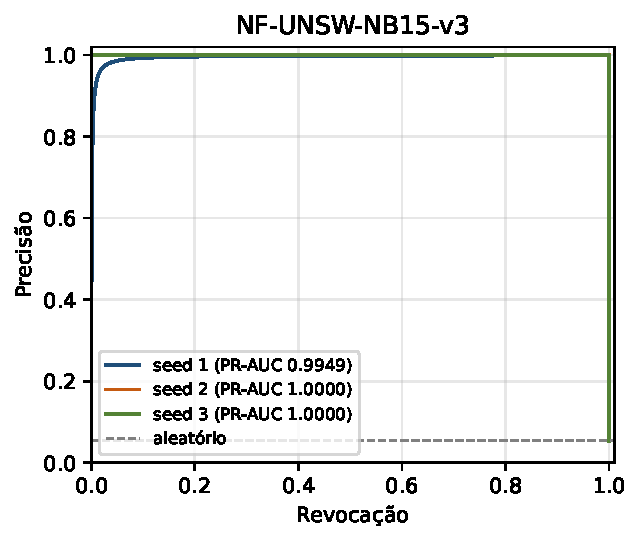
\includegraphics[width=0.49\columnwidth]{NF-UNSW-NB15-v3_pr.pdf}\hfill
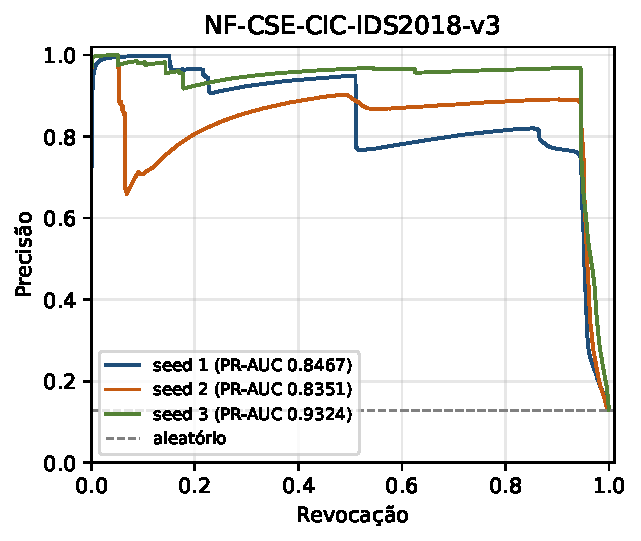
\includegraphics[width=0.49\columnwidth]{NF-CSE-CIC-IDS2018-v3_pr.pdf}\\[2pt]
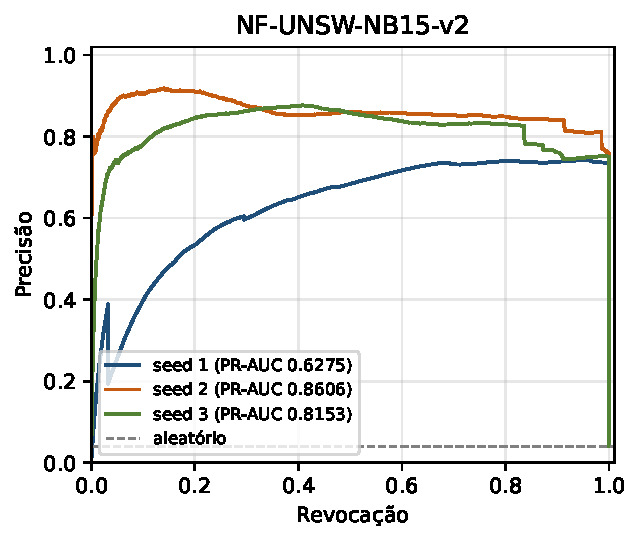
\includegraphics[width=0.49\columnwidth]{NF-UNSW-NB15-v2_pr.pdf}\hfill
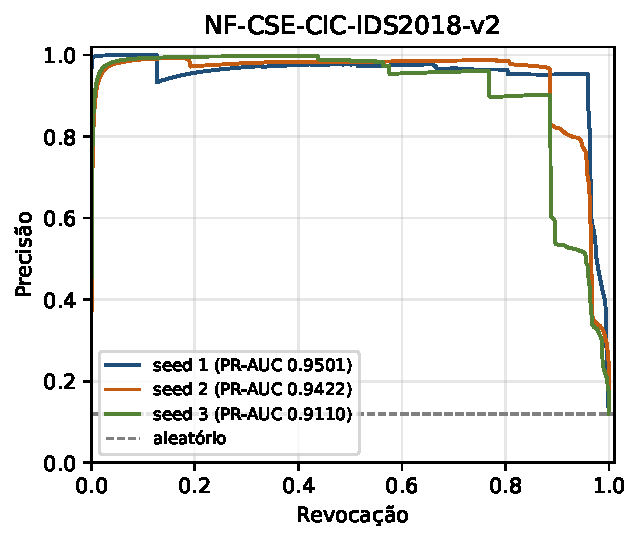
\includegraphics[width=0.49\columnwidth]{NF-CSE-CIC-IDS2018-v2_pr.pdf}
\caption{Curvas precisão-revocação no teste, uma por seed, nos quatro datasets do artigo. A linha tracejada é a de um classificador aleatório (prevalência de ataques).}
\label{fig:pr}
\end{figure}

\textbf{Análise por categoria.} As curvas precisão-revocação
(Figura~\ref{fig:pr}) e as taxas de detecção
(Tabelas~\ref{tab:det_unsw} e~\ref{tab:det_cic}) mostram dois comportamentos
diferentes. No NF-UNSW-NB15-v3 todas as categorias são detectadas em 100\% dos
fluxos, com FPR de 0,003\%, o mesmo comportamento da Figura~5 do artigo. No
NF-UNSW-NB15-v2 todas as categorias passam de 99,5\% de detecção, mas a FPR é de
1,4\%: como há 229.522 fluxos benignos para 9.506 ataques no teste, isso gera cerca
de 3.200 falsos positivos e derruba a precisão para perto de 0,75, o que explica a
PR-AUC menor. O artigo atribui a esse mesmo fator a queda no v2.

\begin{table}[t]
\centering
\caption{Taxa de detecção (\%) por categoria no teste do NF-UNSW-NB15 (média $\pm$ desvio entre seeds). Para os benignos, a taxa é a FPR.}
\label{tab:det_unsw}
\footnotesize
\setlength{\tabcolsep}{3pt}
\begin{tabular}{lrrrr}
\toprule
& \multicolumn{2}{c}{UNSW-NB15-v2} & \multicolumn{2}{c}{UNSW-NB15-v3} \\
\cmidrule(lr){2-3}\cmidrule(lr){4-5}
Categoria & Fluxos & Taxa (\%) & Fluxos & Taxa (\%) \\
\midrule
Benign (FPR) & 229.522 & $1,4 \pm 0,0$ & 223.773 & $0,0 \pm 0,0$ \\
\midrule
Analysis & 230 & $100,0 \pm 0,0$ & 122 & $100,0 \pm 0,0$ \\
Backdoor & 217 & $100,0 \pm 0,0$ & 466 & $100,0 \pm 0,0$ \\
DoS & 580 & $99,7 \pm 0,4$ & 598 & $100,0 \pm 0,0$ \\
Exploits & 3.155 & $99,6 \pm 0,6$ & 4.275 & $100,0 \pm 0,0$ \\
Fuzzers & 2.231 & $99,7 \pm 0,5$ & 3.382 & $100,0 \pm 0,0$ \\
Generic & 1.656 & $100,0 \pm 0,0$ & 1.965 & $100,0 \pm 0,0$ \\
Reconnaissance & 1.278 & $99,8 \pm 0,3$ & 1.708 & $100,0 \pm 0,0$ \\
Shellcode & 143 & $99,5 \pm 0,7$ & 238 & $100,0 \pm 0,0$ \\
Worms & 16 & $100,0 \pm 0,0$ & 16 & $100,0 \pm 0,0$ \\
\bottomrule
\end{tabular}

\end{table}

\begin{table}[t]
\centering
\caption{Taxa de detecção (\%) por categoria no teste do NF-CSE-CIC-IDS2018 (média $\pm$ desvio entre seeds).}
\label{tab:det_cic}
\scriptsize
\setlength{\tabcolsep}{2pt}
\begin{tabular}{lrrrr}
\toprule
& \multicolumn{2}{c}{CIC-IDS2018-v2} & \multicolumn{2}{c}{CIC-IDS2018-v3} \\
\cmidrule(lr){2-3}\cmidrule(lr){4-5}
Categoria & Fluxos & Taxa (\%) & Fluxos & Taxa (\%) \\
\midrule
Benign (FPR) & 332.712 & $0,8 \pm 0,4$ & 350.293 & $3,0 \pm 2,0$ \\
\midrule
Bot & 2.862 & $33,3 \pm 47,1$ & 4.154 & $66,7 \pm 47,1$ \\
Brute Force -Web & 43 & $100,0 \pm 0,0$ & 32 & $100,0 \pm 0,0$ \\
Brute Force -XSS & 18 & $100,0 \pm 0,0$ & 9 & $100,0 \pm 0,0$ \\
DDOS attack-HOIC & 21.618 & $100,0 \pm 0,0$ & 20.646 & $100,0 \pm 0,0$ \\
DDOS attack-LOIC-UDP & 42 & $100,0 \pm 0,0$ & 69 & $100,0 \pm 0,0$ \\
DDoS attacks-LOIC-HTTP & 6.146 & $100,0 \pm 0,1$ & 5.772 & $100,0 \pm 0,0$ \\
DoS attacks-GoldenEye & 555 & $100,0 \pm 0,0$ & 1.226 & $100,0 \pm 0,0$ \\
DoS attacks-Hulk & 8.653 & $100,0 \pm 0,0$ & 2.002 & $100,0 \pm 0,0$ \\
DoS attacks-SlowHTTPTest & 282 & $100,0 \pm 0,0$ & 2.111 & $100,0 \pm 0,0$ \\
DoS attacks-Slowloris & 190 & $100,0 \pm 0,0$ & 721 & $100,0 \pm 0,0$ \\
FTP-BruteForce & 518 & $99,9 \pm 0,1$ & 7.734 & $100,0 \pm 0,0$ \\
Infilteration & 2.328 & $7,2 \pm 9,4$ & 3.763 & $26,7 \pm 4,2$ \\
SQL Injection & 8 & $100,0 \pm 0,0$ & 8 & $100,0 \pm 0,0$ \\
SSH-Bruteforce & 1.900 & $99,9 \pm 0,1$ & 3.770 & $100,0 \pm 0,0$ \\
\bottomrule
\end{tabular}

\end{table}

No NF-CSE-CIC-IDS2018, as categorias de força bruta, DoS e DDoS ficam perto de
100\%, e a perda de desempenho se concentra em duas categorias. A Infiltration é
detectada em só 7\% (v2) e 27\% (v3) dos fluxos, valores próximos dos 18\% e 25\%
do artigo. Esse ataque entrega um payload por e-mail e depois varre a rede interna
a partir do host comprometido, com tráfego muito parecido com o normal; sem
conhecer a assinatura, um detector de anomalias dificilmente o separa do benigno
(Figura~\ref{fig:tsne_artigo}). O Bot apresenta um comportamento bimodal: é
detectado por completo em algumas seeds e quase nada em outras (média de 33\% no v2
e 67\% no v3, com desvio de 47 pontos), o que indica que o limiar escolhido na
validação fica muito perto da distribuição de scores desse ataque
(Figura~\ref{fig:scores_artigo}). Como o Bot e a Infiltration somam cerca de 15\%
dos ataques do teste no v3, eles explicam a maior parte da diferença de PR-AUC
entre o CSE-CIC-IDS2018 e o UNSW-NB15-v3.

\begin{figure*}[t]
\centering
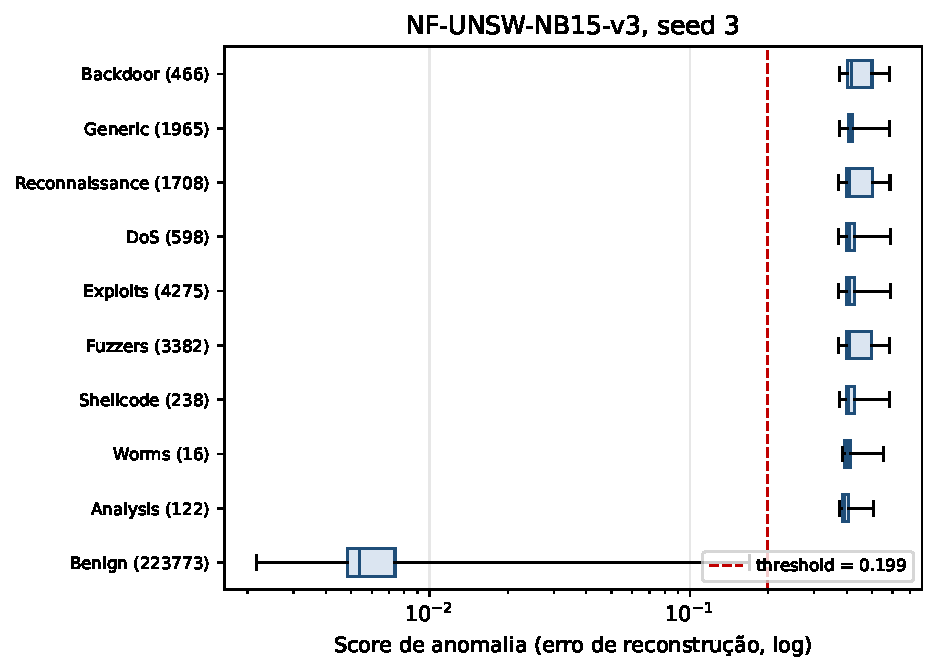
\includegraphics[height=4.6cm]{NF-UNSW-NB15-v3_scores.pdf}\qquad
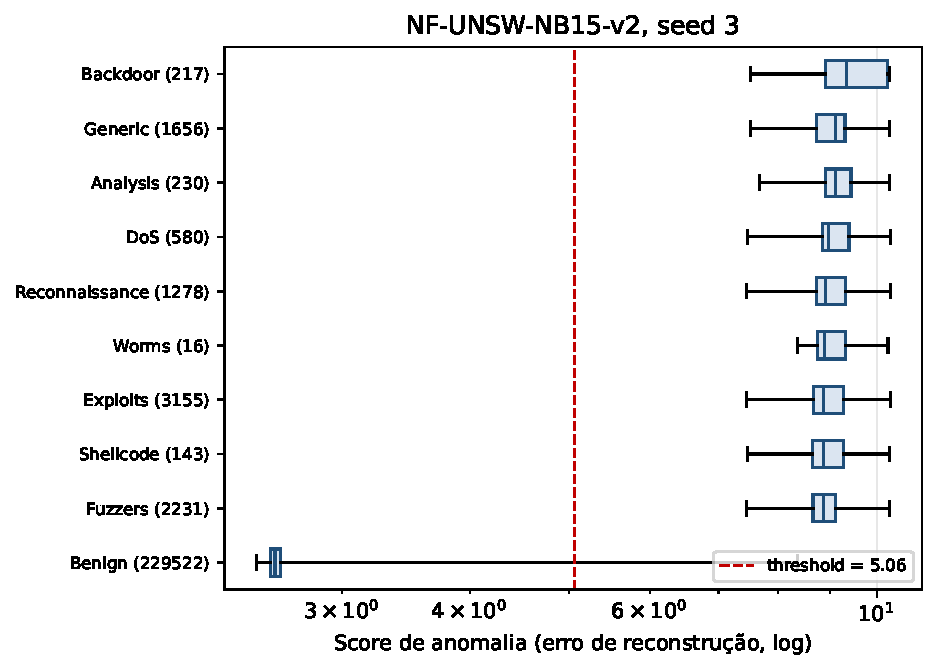
\includegraphics[height=4.6cm]{NF-UNSW-NB15-v2_scores.pdf}\\[4pt]
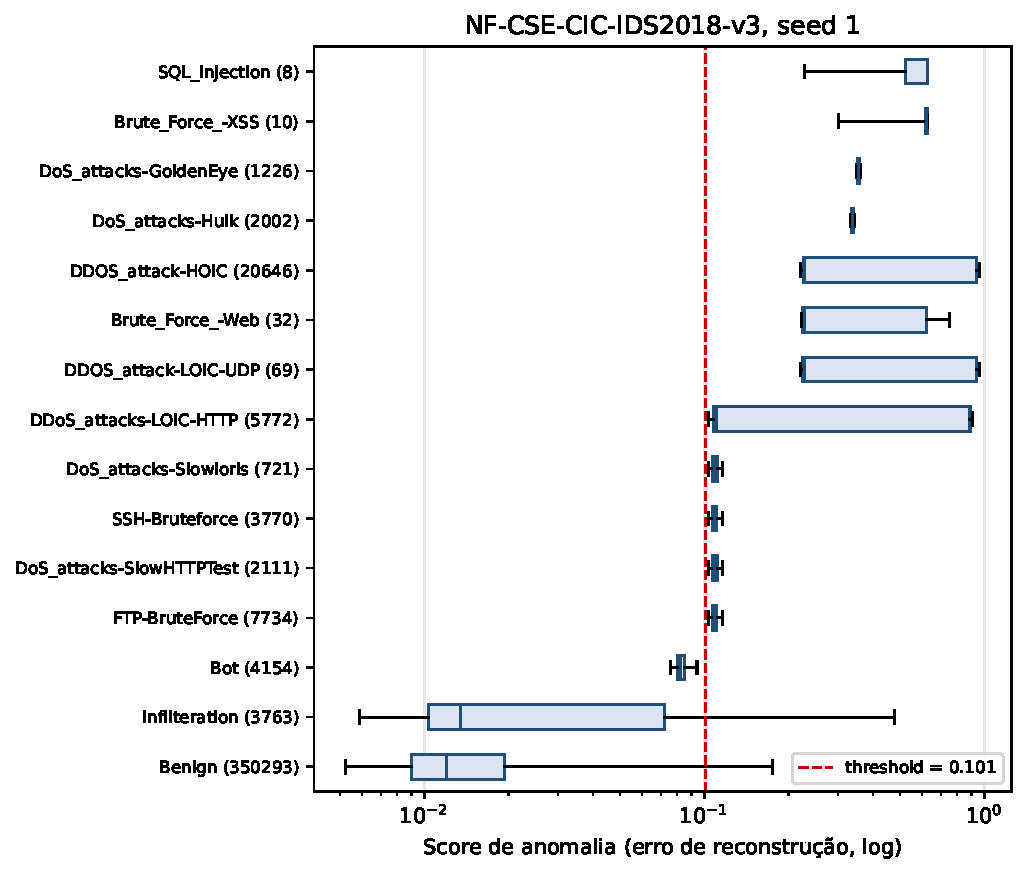
\includegraphics[height=4.6cm]{NF-CSE-CIC-IDS2018-v3_scores.pdf}\qquad
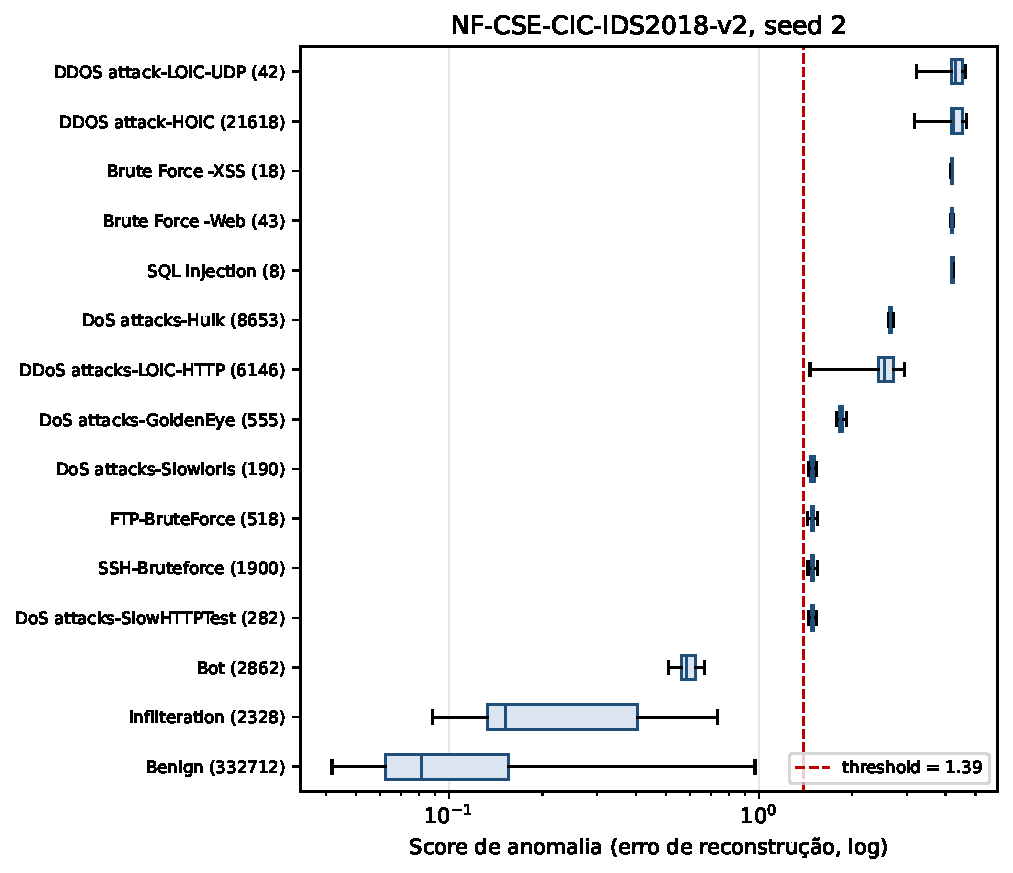
\includegraphics[height=4.6cm]{NF-CSE-CIC-IDS2018-v2_scores.pdf}
\caption{Distribuição do score de anomalia (escala log) por categoria no teste, com o limiar escolhido na validação (linha vermelha), em uma seed representativa de cada dataset do artigo. Categorias à direita do limiar são detectadas.}
\label{fig:scores_artigo}
\end{figure*}

\begin{figure*}[t]
\centering
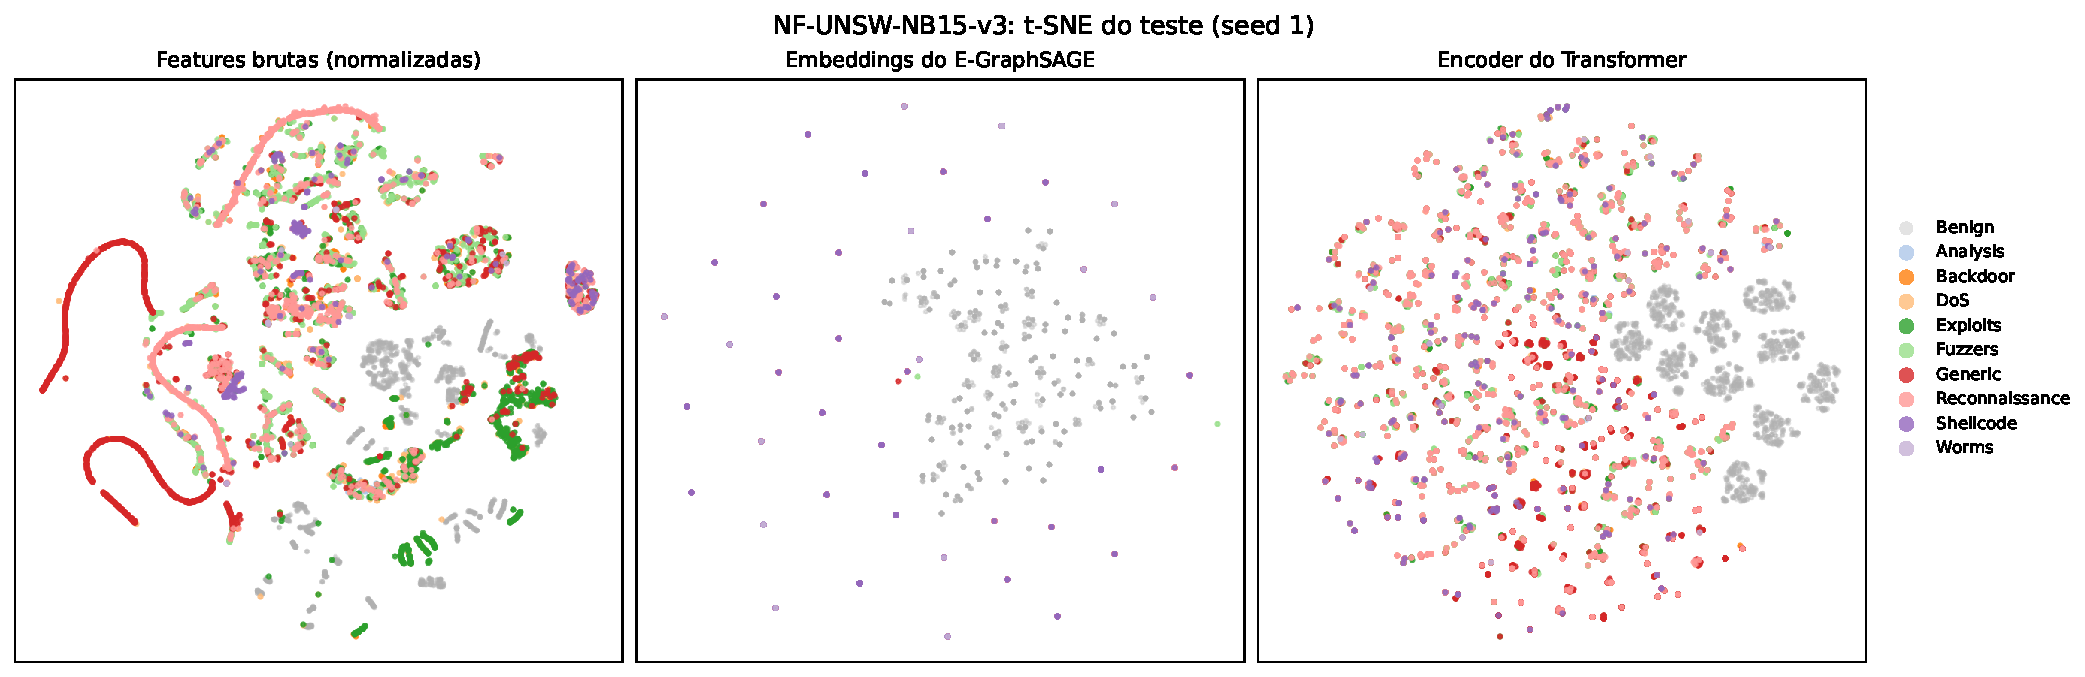
\includegraphics[width=0.49\textwidth]{NF-UNSW-NB15-v3_tsne.pdf}\hfill
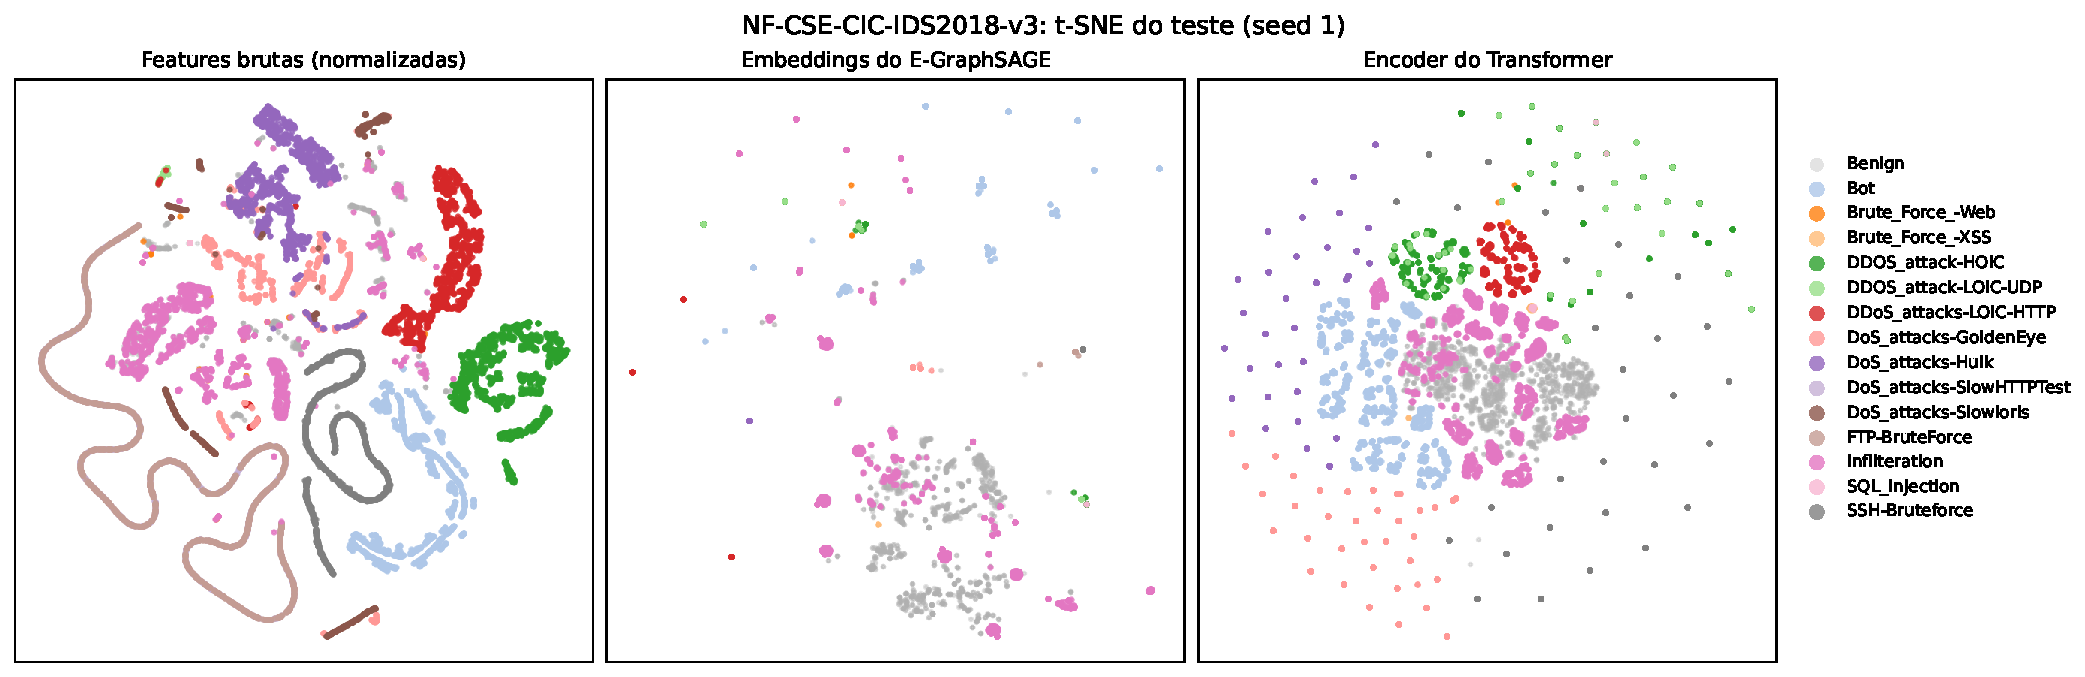
\includegraphics[width=0.49\textwidth]{NF-CSE-CIC-IDS2018-v3_tsne.pdf}
\caption{t-SNE~\cite{vandermaaten2008tsne} das features normalizadas, dos embeddings do E-GraphSAGE e da saída do encoder do Transformer no teste (seed 1), para o NF-UNSW-NB15-v3 (esquerda) e o NF-CSE-CIC-IDS2018-v3 (direita).}
\label{fig:tsne_artigo}
\end{figure*}

\textbf{Custo computacional.} A Tabela~\ref{tab:custo} compara o custo da nossa
implementação com a Tabela~2 do artigo. Nosso modelo tem de 0,058 a 0,100 milhão
de parâmetros, contra 0,570 a 0,874 milhão no artigo, com os mesmos
hiperparâmetros da Tabela~14. A diferença deve vir de algum componente que a
contagem do artigo inclui e a nossa não (por exemplo, uma camada
\emph{feed-forward} maior na versão usada para os números publicados); não
conseguimos identificá-lo, mas, como os resultados ficaram próximos, ele não parece
ser essencial ao desempenho. O treino levou de 2,5 a 8,7 minutos em média, contra
23 a 88 minutos no artigo, e a inferência, de 0,24 a 0,82~$\mu$s por fluxo, contra
2,27 a 5,09~$\mu$s. Parte dessa diferença vem do modelo menor e da agregação
pré-calculada, e parte do \emph{early stopping}, que parou várias execuções cedo.
O pico de memória da GPU ficou entre 0,9 e 1,3~GB, próximo dos 1,37~GB médios do
artigo. Os tempos devem ser comparados com cautela, porque algumas execuções podem
ter caído numa fatia MIG da A100.

\begin{table*}[t]
\centering
\caption{Custo computacional (média $\pm$ desvio entre seeds), comparado com a Tabela 2 do artigo. A inferência mede só a passagem direta, sem pré-processamento.}
\label{tab:custo}
\footnotesize
\begin{tabular}{l rr rr rr r}
\toprule
& \multicolumn{2}{c}{Parâmetros (M)} & \multicolumn{2}{c}{Treino (min)} & \multicolumn{2}{c}{Inferência ($\mu$s/fluxo)} & Mem. GPU \\
\cmidrule(lr){2-3}\cmidrule(lr){4-5}\cmidrule(lr){6-7}
Dataset & nosso & artigo & nosso & artigo & nosso & artigo & (MB) \\
\midrule
UNSW-NB15-v3 & 0,100 & 0,874 & $8,7 \pm 3,5$ & $37,8 \pm 19,2$ & $0,76 \pm 0,57$ & $3,04 \pm 1,25$ & 901 \\
CIC-IDS2018-v3 & 0,059 & 0,572 & $8,7 \pm 4,1$ & $87,6 \pm 35,4$ & $0,44 \pm 0,00$ & $5,09 \pm 1,09$ & 1.201 \\
UNSW-NB15-v2 & 0,093 & 0,867 & $2,5 \pm 0,9$ & $23,4 \pm 16,2$ & $0,24 \pm 0,00$ & $2,27 \pm 0,92$ & 1.260 \\
CIC-IDS2018-v2 & 0,058 & 0,570 & $7,8 \pm 6,5$ & $60,0 \pm 33,0$ & $0,69 \pm 0,20$ & $4,89 \pm 0,50$ & 1.068 \\
\midrule
ToN-IoT-v3 & 0,100 & -- & $5,4 \pm 2,7$ & -- & $0,82 \pm 0,24$ & -- & 1.175 \\
\bottomrule
\end{tabular}

\end{table*}

\subsection{Solução do artigo de referência no NF-ToN-IoT-v3}

\textbf{Desempenho geral.} No NF-ToN-IoT-v3 o GraphIDS obtém PR-AUC de
$0{,}6872\pm0{,}0192$ e F1 macro de $0{,}6408\pm0{,}1488$
(Tabela~\ref{tab:ton}). A PR-AUC fica 1,8 vez acima da linha de base aleatória
(0,3898), então o modelo aprende algo útil, mas o resultado é muito inferior ao dos
datasets do artigo, em que a PR-AUC fica de 6,7 a 19,3 vezes acima da linha de
base. Não há resultados publicados do GraphIDS nem dos baselines do artigo neste
dataset, por isso a comparação é com os datasets do artigo e com essa linha de
base. O F1 macro varia muito entre seeds (0,7468, 0,7049 e 0,4707), e a seed~3 já
tinha F1 macro de 0,4666 na validação, ou seja, o limiar que maximiza o F1 não
consegue separar bem as classes naquele checkpoint.

\begin{table}[t]
\centering
\caption{Desempenho no teste (média $\pm$ desvio) e PR-AUC de referência de um classificador aleatório ($^\ast$prevalência de ataques no teste).}
\label{tab:ton}
\footnotesize
\setlength{\tabcolsep}{3pt}
\begin{tabular}{lccc}
\toprule
Dataset & PR-AUC & F1 macro & \makecell{PR-AUC de\\referência$^\ast$} \\
\midrule
UNSW-NB15-v3 & $0,9983 \pm 0,0029$ & $0,9999 \pm 0,0001$ & 0,0540 \\
CIC-IDS2018-v3 & $0,8714 \pm 0,0531$ & $0,9252 \pm 0,0435$ & 0,1293 \\
UNSW-NB15-v2 & $0,7678 \pm 0,1236$ & $0,9232 \pm 0,0038$ & 0,0398 \\
CIC-IDS2018-v2 & $0,9344 \pm 0,0207$ & $0,9567 \pm 0,0179$ & 0,1195 \\
\midrule
ToN-IoT-v3 & $0,6872 \pm 0,0192$ & $0,6408 \pm 0,1488$ & 0,3898 \\
\bottomrule
\end{tabular}

\end{table}

\textbf{Análise por categoria.} A Tabela~\ref{tab:det_ton} e a
Figura~\ref{fig:ton}(a) mostram que o desempenho depende muito do tipo de
ataque. Backdoor e ransomware são detectados em 100\% dos fluxos em todas as
seeds, e injection em 68\%. Já DDoS (50\%), password (43\%), XSS (40\%), DoS (36\%) e
MITM (34\%) ficam abaixo da metade, com desvios de 17 a 36 pontos entre seeds, e o
scanning é detectado em apenas 4\%, mesmo sendo a categoria com assinatura
topológica mais clara no modelo de ameaça. A FPR é de 9,9\%, cerca de dez vezes a
dos datasets do artigo, porque o limiar precisa ser baixo para capturar parte dos
ataques. Na Figura~\ref{fig:ton}(a), a distribuição de scores do scanning fica à
\emph{esquerda} da dos benignos: o modelo reconstrói esses fluxos melhor do que o
próprio tráfego normal.

\begin{table}[t]
\centering
\caption{Taxa de detecção (\%) por categoria no teste do NF-ToN-IoT-v3 (média $\pm$ desvio entre seeds).}
\label{tab:det_ton}
\footnotesize
\begin{tabular}{lrr}
\toprule
Categoria & Fluxos & Taxa (\%) \\
\midrule
Benign (FPR) & 335.845 & $9,9 \pm 7,3$ \\
\midrule
Backdoor & 4.067 & $100,0 \pm 0,0$ \\
ddos & 82.825 & $49,8 \pm 36,0$ \\
dos & 4.069 & $36,4 \pm 25,7$ \\
injection & 7.636 & $67,7 \pm 17,3$ \\
mitm & 120 & $34,4 \pm 36,5$ \\
password & 31.896 & $43,4 \pm 29,6$ \\
ransomware & 79 & $100,0 \pm 0,0$ \\
scanning & 27.180 & $4,2 \pm 5,0$ \\
xss & 56.689 & $40,5 \pm 20,5$ \\
\bottomrule
\end{tabular}

\end{table}

\begin{figure*}[t]
\centering
\begin{minipage}[b]{0.30\textwidth}
\centering
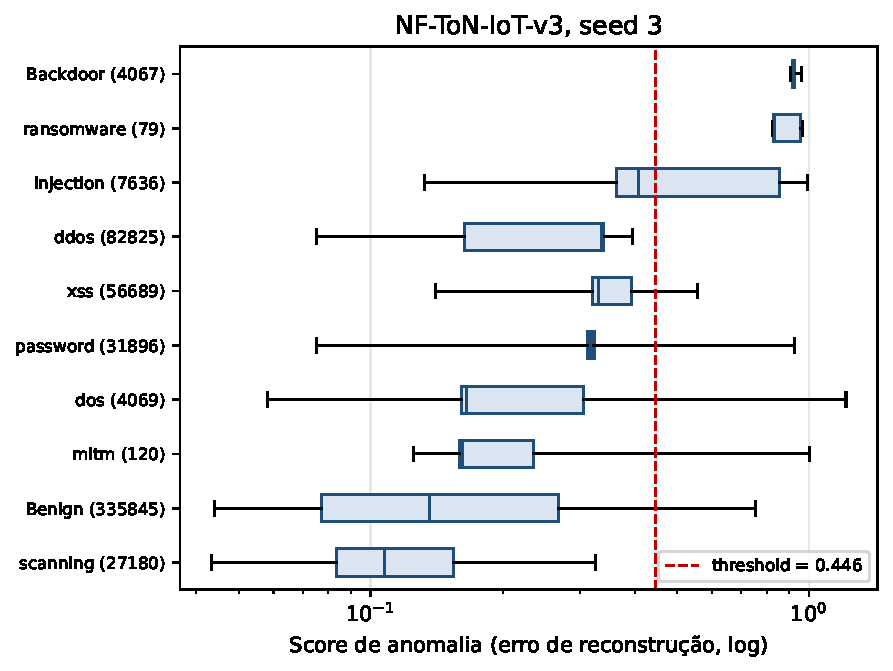
\includegraphics[width=\linewidth]{NF-ToN-IoT-v3_scores.pdf}\\
\scriptsize (a)
\end{minipage}\hfill
\begin{minipage}[b]{0.42\textwidth}
\centering
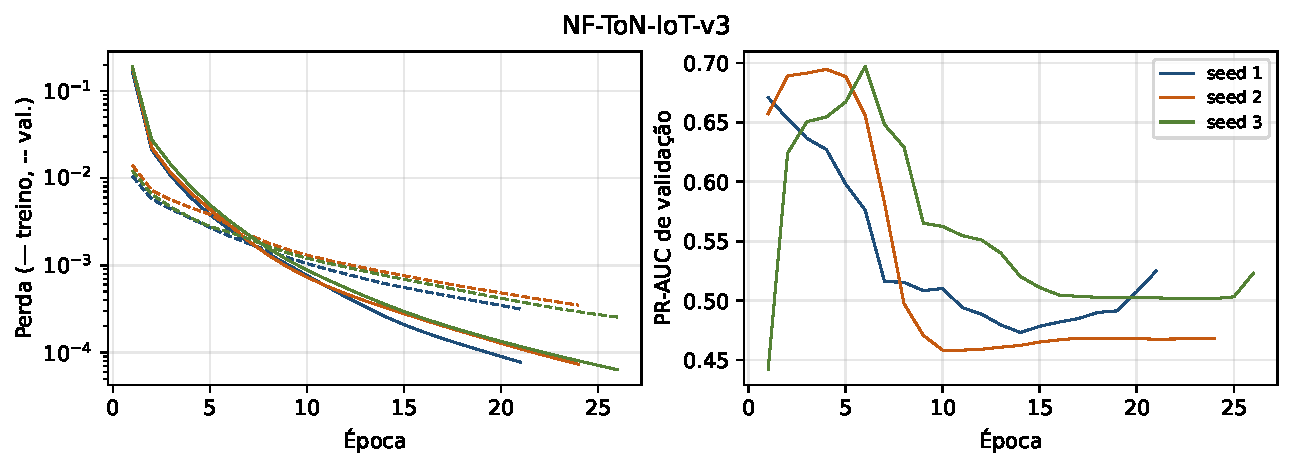
\includegraphics[width=\linewidth]{NF-ToN-IoT-v3_treino.pdf}\\
\scriptsize (b)
\end{minipage}\hfill
\begin{minipage}[b]{0.24\textwidth}
\centering
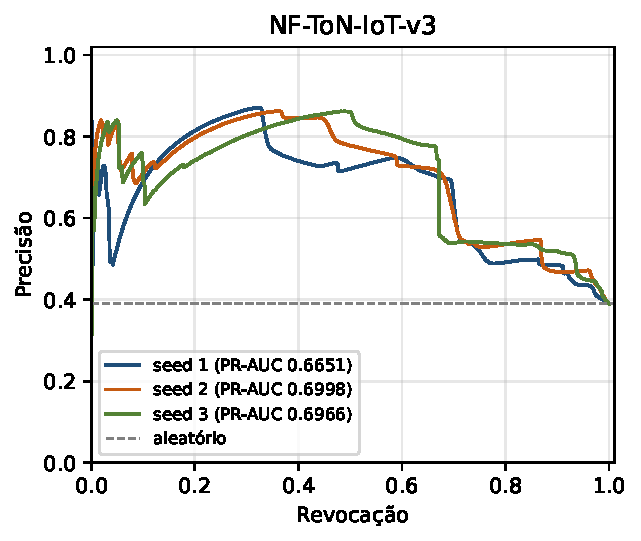
\includegraphics[width=\linewidth]{NF-ToN-IoT-v3_pr.pdf}\\
\scriptsize (c)
\end{minipage}\\[4pt]
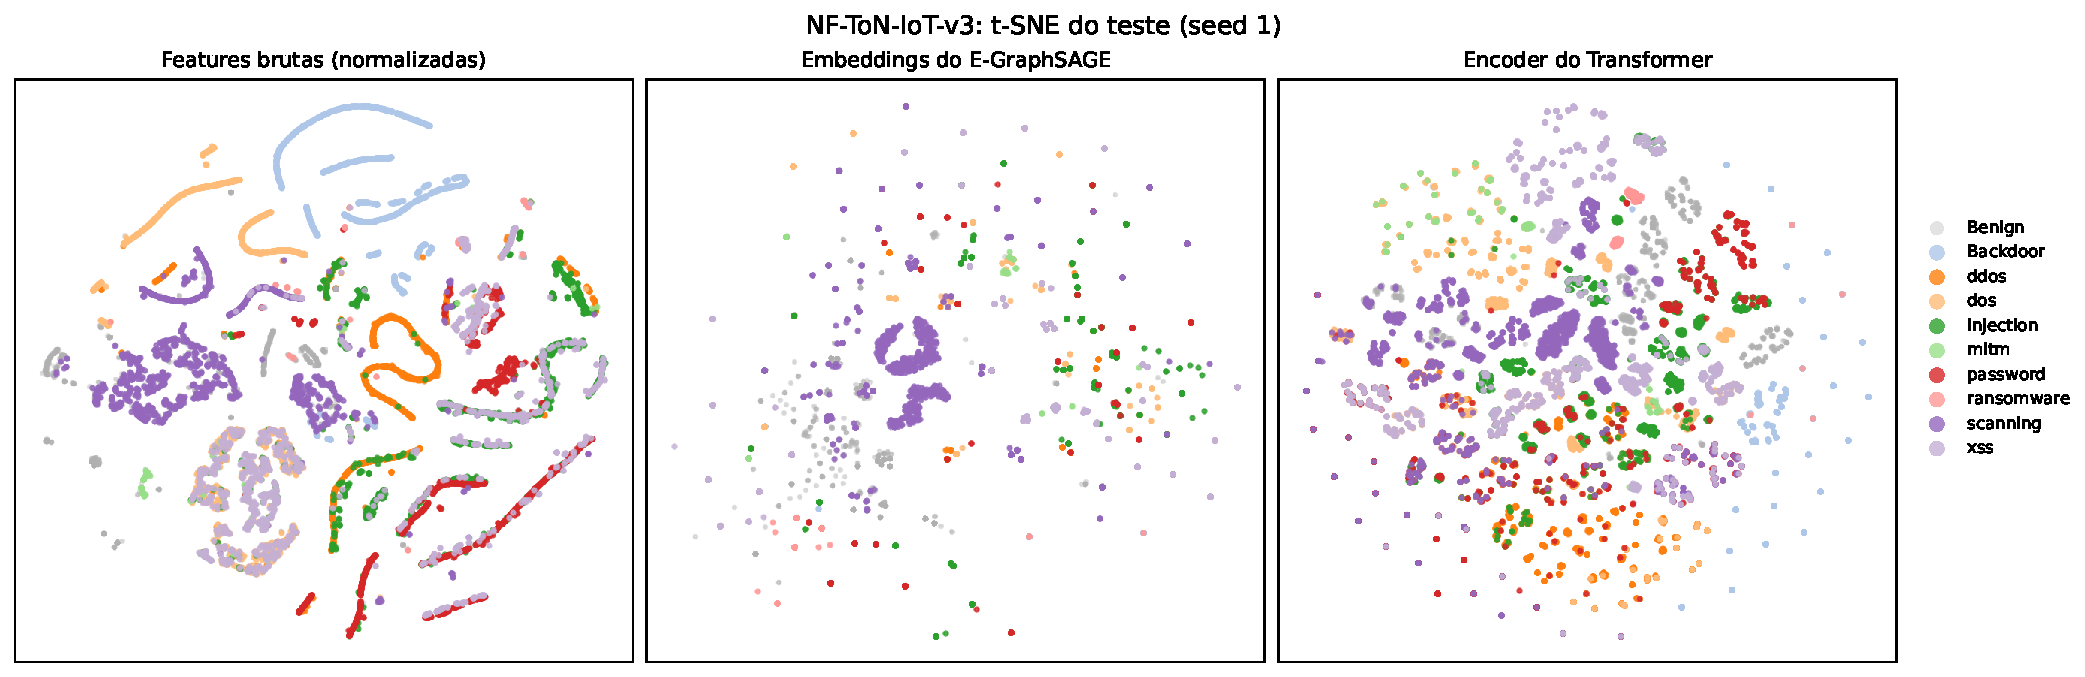
\includegraphics[width=0.9\textwidth]{NF-ToN-IoT-v3_tsne.pdf}\\
\scriptsize (d)
\caption{NF-ToN-IoT-v3: (a) distribuição do score por categoria no teste, com o limiar (seed 3); (b) perda de treino e validação (esquerda) e PR-AUC de validação (direita) por época; (c) curvas precisão-revocação no teste; (d) t-SNE das features, dos embeddings do E-GraphSAGE e da saída do encoder (seed 1).}
\label{fig:ton}
\end{figure*}

\textbf{Por que o desempenho cai.} Os nossos dados apontam três causas, que se
somam:
\begin{enumerate}
  \item \emph{Desalinhamento entre reconstrução e detecção.} Na
        Figura~\ref{fig:ton}(b), a perda de reconstrução cai durante todo o
        treino, mas a PR-AUC de validação atinge o máximo entre as épocas 1 e 6
        e depois cai para cerca de 0,47 a 0,52. Por isso o melhor checkpoint
        foi o da época 1, 4 e 6 nas três seeds (Tabela~\ref{tab:seeds}), contra
        as épocas 5 a 96 nos datasets do artigo. O modelo fica cada vez melhor
        em reconstruir \emph{qualquer} fluxo, inclusive os de ataque, e o erro
        de reconstrução deixa de separar as classes. Fluxos de scanning, curtos
        e muito regulares, são o caso extremo.
  \item \emph{Ataques e tráfego benigno compartilham hosts.} O grafo tem poucos
        hosts para muitos fluxos (6.355 hosts para 2,7 milhões de fluxos no
        treino). Pelas Eqs.~(\ref{eq:agg}) e~(\ref{eq:edge}), o embedding de um
        fluxo $u\to v$ depende apenas das médias das arestas que chegam em $u$ e
        em $v$, com até 32.768 arestas por host; a feature do próprio fluxo só
        entra diluída nessa média. Quando um ataque usa os mesmos hosts que o
        tráfego normal, o seu embedding fica muito parecido com o dos fluxos
        benignos entre os mesmos hosts. O t-SNE da Figura~\ref{fig:ton}(d)
        ilustra isso: nas features brutas várias categorias formam grupos
        bem definidos, enquanto nos embeddings do E-GraphSAGE elas aparecem
        muito mais misturadas aos benignos. Nos datasets do artigo, ao contrário, os ataques tendem a
        envolver hosts e padrões de conexão próprios.
  \item \emph{Sem ajuste de hiperparâmetros.} Usamos a configuração do
        NF-UNSW-NB15-v3 sem nenhum ajuste, enquanto o artigo faz busca em grade e
        otimização bayesiana para cada dataset. Em particular, a taxa de
        aprendizado de $10^{-4}$ faz o modelo convergir em poucas épocas, o que
        acelera o desalinhamento descrito no item~1.
\end{enumerate}
A alta prevalência de ataques (39\%) também pesa: a premissa de que anomalias são
raras e diferentes do normal fica mais fraca quando quase quatro em cada dez
fluxos são ataques, muitos deles com volume parecido ao do tráfego benigno.

\subsection{Proposta da equipe}

Como explicado na Seção~\ref{sec:proposta}, a equipe não implementou modificações
no GraphIDS, então não há resultados de uma versão melhorada nos dados do artigo
nem no NF-ToN-IoT-v3.

% ----------------------------------------------------------------------------
\section{Conclusão e trabalhos futuros}
\label{sec:conclusao}

Reimplementamos do zero o GraphIDS, um NIDS auto-supervisionado que treina de
ponta a ponta um E-GraphSAGE e um autoencoder Transformer com máscara de atenção
para reconstruir representações de tráfego benigno. Nos quatro datasets do
artigo, a reprodução ficou a até dois desvios-padrão dos valores publicados em 7
das 8 métricas, e confirmou que o método supera com folga os baselines externos
nos datasets v3. A nossa implementação tem cerca de um décimo dos parâmetros
reportados e treina em minutos, com desempenho equivalente.

No NF-ToN-IoT-v3, um ambiente IoT/IIoT com 39\% de ataques, o desempenho caiu para
PR-AUC de 0,6872 e F1 macro de 0,6408. Backdoor e ransomware são sempre
detectados, mas scanning, DoS, DDoS, XSS e ataques de senha são, em grande parte,
reconstruídos tão bem quanto o tráfego normal.

\textbf{Limitações do sistema do artigo.} (i) O limiar e o \emph{early
stopping} usam uma validação rotulada, o que contraria em parte a proposta de
não depender de rótulos de ataque, e o F1 é sensível a esse limiar (caso do Bot e
da seed~3 do ToN-IoT). (ii) A reconstrução não garante separação: quando os
ataques são frequentes ou regulares, o autoencoder aprende a reconstruí-los, e a
PR-AUC de validação piora enquanto a perda melhora. (iii) O embedding do fluxo
depende só da vizinhança dos dois hosts, então ataques que compartilham hosts com
o tráfego normal, como Infiltration e boa parte do ToN-IoT, ficam pouco
distinguíveis. (iv) O método assume comportamento normal estável, sem mudanças
bruscas de distribuição, e não foi avaliado contra atacantes adaptativos ou
envenenamento do treino (premissas P4 e P5). (v) O desempenho varia bastante
entre seeds em alguns datasets e depende de ajuste fino por dataset.

\textbf{Limitações deste trabalho.} Não reexecutamos os baselines e usamos os
números do artigo; avaliamos três seeds; não ajustamos os hiperparâmetros para o
NF-ToN-IoT-v3; e não identificamos a origem da diferença no número de
parâmetros.

\textbf{Trabalhos futuros.} Os resultados sugerem, em ordem de prioridade:
(1) ajustar taxa de aprendizado, \emph{dropout} do GNN e \texttt{edim\_out} no
NF-ToN-IoT-v3 pela PR-AUC de validação; (2) incluir as features do próprio fluxo
no embedding, por exemplo concatenando $\vect{x}_{uv}$ a
$[\vect{h}_u\Vert\vect{h}_v]$ na Eq.~(\ref{eq:edge}), para que ataques entre hosts
benignos se distingam; (3) usar um limiar não supervisionado, como mediana mais
um múltiplo do desvio absoluto mediano dos scores benignos, e um critério de
parada que não dependa de rótulos; (4) avaliar o grafo completo do
CSE-CIC-IDS2018, janelas temporais de grafo e robustez a evasão e a
envenenamento dos dados de treino.

% ----------------------------------------------------------------------------
\bibliographystyle{IEEEtran}
\bibliography{referencias}

\end{document}
